\chapter{Internet-of-Money: Real-time Money Routing by Trusting Strangers with your Funds}
\label{chapter:iom}

\emph{We explore a new stage in the evolution of digital trust, trusting strangers with your funds.
We address the trust issues when giving money to others and relying on them to forward it.
For fraud identification, we leverage our deployed blockchain which gradually builds trust between interacting strangers.
Our blockchain fabric, called \emph{TrustChain}, records interactions between entities in a scalable manner.
This work represents a small step towards a generic infrastructure for trust, moving beyond proven single vendor platforms like eBay, Uber and Airbnb.}

\emph{In this chapter we design, implement and evaluate an overlay network: \emph{Internet-of-Money}.
Internet-of-Money routes money to different banks through individuals, so-called \emph{money routers}.
This removes the need for central banks, to handle a payment.
Our network reduces the duration of traditional inter-bank payments from up to a day and even a few days during weekends, to mere seconds.
Internet-of-Money is fully decentralized, scalable and privacy-preserving.}

\emph{With real-world experimentations, we prove that Internet-of-Money enables fast money forwarding.
We show that the overlay network is capable of discovering a majority of available money routers within a minute.
Finally, we demonstrate how profit of cheating routers is limited and that misbehaviour is punished.}

\newpage

\section{Introduction}
% One of the first systems, craigslist, unmoderated... 
Creating trust between strangers is at the core of numerous successful Internet companies.
Starting 22 years ago, Craigslist offered an unmoderated mailing list of advertisements and gossip on which buyer and seller could be trusted.
eBay formalised this in 1997 and introduced a star-based rating system that enables traders to build a trustworthy profile~\cite{resnick2002trust}.
The e-commerce platform was launched at a time when people were still hesitant to use their credit card on a technology called The Internet.
Nowadays, people let strangers sleep in their houses using Airbnb (since 2008).
We trust Uber (since 2009) with our physical security and get into cars late at night with a driver that has never undergone a criminal background check or given a government license.
%Airbnb transformed the notion of letting strangers sleep in your house from an uncomfortable idea to a viable business model.
These influential milestones in the evolution of digital trust are shown in Figure \ref{fig:trust_evolution}.

We continue this evolution of building trust.
We created an operational platform for one of the most challenging and sensitive applications, having others handle your money.

Bitcoin created money without the need for banks~\cite{nakamoto2008bitcoin}.
In the past, people were required to trust a central bank and a host of other intermediaries when making payments~\cite{kokkola2011payment}.
The fundamental technology of Bitcoin, blockchain, radically reduced the need to trust financial middlemen.
It bootstrapped an economy where no one can be stopped from spending their money.
Despite widespread speculation and ecosystems being worth billions, blockchain in general suffers from scalability issues due to inefficient mechanisms for fraud prevention.
Bitcoin is theoretically limited to seven transactions per second and Ethereum has a throughput of around twenty transactions per second~\cite{vukolic2015quest}.
Despite various scalability efforts like proof-of-stake and sharding, broader adoption of blockchain stays out.
%Broader adoption is limited since blockchain applications are fragmented with low interoperability.

\begin{figure*}[!t]
	\centering
	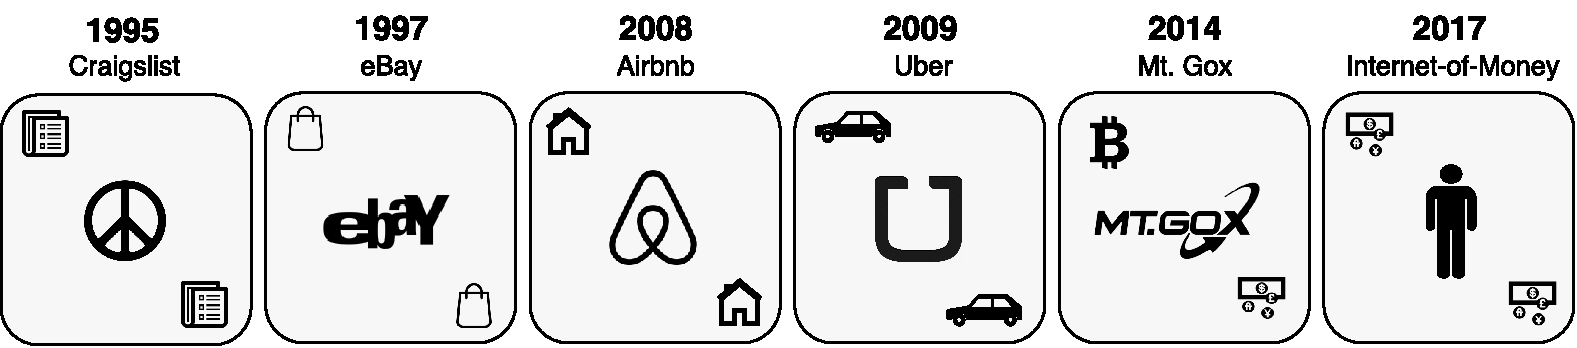
\includegraphics[width=\linewidth]{iom/assets/timeline}
	\caption{Influential milestones in the evolution of digital trust.}
	\label{fig:trust_evolution}
\end{figure*}

%A majority of Internet usage takes place on handful of platforms that are operated by large companies.
While a majority of Internet users trust the company behind popular platforms, the events involving Mt. Gox highlighted how digital trust can be established and compromised~\cite{mcmillan2014inside}.
Mt. Gox was at one point the largest Bitcoin exchange worldwide.
In 2014, hackers stole Bitcoin, worth around \$460 million at that time. %Mt. Gox, at that time the largest Bitcoin exchange operational.
This event, together with major data breaches in 2017 at high-profile companies like Uber and Equifax, exposed the weakness of centralized architectures~\cite{uber2017hack}.
They motivate research around decentralized technologies, like blockchain. %, not owned or operated by a single authority.
%Other data breaches challenge high-profile companies like Uber and Equifax to consider their 

%We explore a new stage in the evolution of digital trust and address the challenging problem of \emph{how to trust strangers with your money}.
The generic problem of building trust between strangers resides on the edge of technology, sociology and behavioural science~\cite{yan2008trust}.
%Our work devises a protocol for creating trust.
The question whether someone can be trusted, depends on properties like personality, level of authority, culture and past behaviour. % https://www.researchgate.net/publication/267260663_Social_Trust_A_Cognitive_Approach
In this research, we address the trust problem from a technological perspective, using tamper-proof interactions on a scalable blockchain.
This structure is built to detect fraudulent behaviour and misrepresentation.
%This work demonstrates how to build trust between strangers in such a way that we can trust others with your funds.
We explore whether a trust model based merely on historical encounters is sufficient to trust strangers with your money.

With established trust relations, we demonstrate how one can transfer money within seconds between different banks by relying on others to act as financial intermediaries.
In comparison to most proven platforms, our solution is designed to be fully decentralized and autonomous. %, similar to the design principles of The Internet itself.
Our work is motivated by slow money transfers to other banks using existing systems. %and high costs when moving funds cross-border.
Inter-banking payments often take up to a day or even a few days during weekends to arrive in the account of a beneficiary.

The main contributions of this work are as follows:
\begin{enumerate}
	\item A trust model, based on repeated interactions and stored on a tamper-proof, scalable blockchain.
	\item \emph{Internet-of-Money}, a novel overlay network that allows real-time money routing to other banks.
	\item Experimental quantification of the performance of our trust model, the speed of money transfers and the efficiency of our overlay network.
	\item A framework to interface with multiple banks and to initiate payments to others using Internet-of-Money.
	% \item An Android application, capable of transferring money to other bank accounts within seconds.
\end{enumerate}

%The Internet shaped dynamics of human interaction and therefore, altered how trust relations are commenced and maintained.
%The ubiquitous, open nature of the Internet allows strangers to interact, collaborate or trade from anywhere on the world, at any time.
%Wide-spread adoption of mobile technology permits individuals to be part of a digital community and manage relations, both in a professional and personal context, without immediate access to a personal computer.
%Social networks like Facebook, Twitter and LinkedIn lower the barrier for people to meet and interact with strangers.
%Nowadays, a large part of our social lives resolves around maintaining digital connections with family, friends and colleagues.

%Figure \ref{fig:trust_evolution} highlights influential milestones in the evolution of digital trust.
%Craigslist is one of the earliest platforms operating on the Internet that provides utility to users beyond discussion by digitalizing advertisements that usually were placed in traditional media like newspapers or journals.
%Craigslist was founded in 1995 and is operational in 70 countries as of 2017.

% Directed trading using a trusted intermediary
%In the same year, eBay built a digital platform that allows online sales between customers and businesses. % was founded and boomed the popularity of e-commerce activities on the Internet by facilitating auctions between strangers.
%Whereas users traditionally had to meet in person to make sure that the other party acts legitimate and can be trusted, eBay removed the geographical requirement for actions and generic trade.
%The platform pioneered the concept of e-commerce, today a market worth billions.
%Trust between traders is established by leaving public feedback on the platform, effectively creating a trace of past transactions for each trader.
%In turn, each trader has a personal log of historical transactions and feedback associated with each transaction.
%Before e-commerce became mainstream, individuals had to rely on newspapers and had to meet face-to-face to make sure that the other party acts legitimate.

%The next milestone in digital trust resolves around collaborative consumption within \emph{the sharing economy}.
%Companies like Airbnb (2008, house sharing) and Uber (2009, ride hailing), advanced trust relations and facilitate service exchange through digital platforms.
%Similar to eBay, trustworthiness of participants is quantified by a public reputation mechanism where transacting parties rate each other and leave reviews.
%Most services operating in the sharing economy are offered by centralized entities, responsible for managing trust relations.

%The introduction of Airbnb in 2008 and Uber in 2009 defined a new stage in digital trust: \emph{the sharing economy}.
%Users use the Airbnb platform to let potential strangers sleep in their houses or to find an accommodation.
%Uber provides online ride-hailing services where people can offer or request transportation to a remote location.

%In 2014, over an half million Bitcoins were compromised on the Mt. Gox cryptocurrency exchange by hackers.
%This violation of trust highlighted one of the weaknesses of centralized architectures and catalysed the motivation for decentralized exchanges, not owned or operated by a single authorization.

%In 2016, OpenBazaar got introduced, facilitating peer-to-peer trading between users without relying on a centralized authority that maintains trust relation.
%In OpenBazaar, users are free to open their personal store and sell goods to others.
%The decentralized platform is powered by blockchain technology.
%Blockchain technology holds the promise to redefine the way the economy works by providing trust when transacting with individuals that are inherently untrusted.
%Various successful platforms like Bitcoin and Ethereum has shown the viability of blockchain to build a trustful environment, without a central point of control.

\section{Problem Description}
Trust and fraud are essential problems to address when trusting others with your money. % let them forward it.
%These problems stem from the incentive to keep money sent to you by strangers. 
%We aim to bring digital trust to the next level by exploring how we can rely on others to hold on our funds and eventually forward it to others.
While most cryptocurrencies use a lottery system to stumble upon trustful executors, we rely on game theory to ensure honest behaviour has the largest rewards.
We focus on the effective detection and punishment of fraudulent behaviour.
While it is a common belief that money transfer systems should be safe against all kinds of fraud, we argue that it is sufficient for fraud to be detectable and punishable.
This is comparable to the operation of credit card companies, which have to deal with a considerable amount of fraud on a daily basis.
Detection of such fraud is non-trivial.
%Real-time detection of credit card fraud is non-trivial.

%Our system is specifically designed where honest behaviour consistently has the largest reward,
%To this end, we assume a simple but generic \emph{send and forward} model where a specific entity first sends funds to someone else and then instructs him to forward it. % handle according to your instructuions/handle as instructed
%The receiver of the funds now holds the money until an event is observed with specifications to forward the received money to someone else.
%The essential problem to address now is \emph{how to trust strangers with your money and rely on them to forward it}.
%The requirement for trust stems from the incentive by intermediaries to not forward the money to another bank account and keep the money.
%In particular, our design should punish intermediaries who act malicious.

% Broad research area, not solved yet, hard problem, fake accounts in facebook, twitter (low costs Sybil attack)
% 36000 twitter accounts have been found linked to Russia and Ukrain, for future use

%We believe the solution for this problem lies in a public and decentralized reputation mechanism that assigns trustworthiness scores to individuals, based on past interactions.
%While reputation systems are highly in use, however, a high reputation does not prevent users from abusing their standing.
%For instance, a user can first build a high reputation by acting honest for a long period of time and use this reputation to abuse a trust relation in such a way that it benefits this user.
%This is also referred to as the \enquote{pump and dump} method.
%Another challenging attack in decentralized networks is the Sybil Attack, where an individual creates multiple fake identities and initiate transactions with them to increase his or her reputation.
%The Sybil Attack is often prevented by introducing trusted third parties (TTPs), responsible for validating identities that join the network.

The trust problem in this work can be modelled by the prisoner's dilemma, where two entities can either cooperate or betray each other~\cite{kreps1982rational}.
Betrayal is also called \emph{defection}.
In the iterative prisoner's dilemma, players cooperate or deflect iteratively and are able to punish opponents for their past decisions.
We assume a \emph{send and forward} model where a user first sends money to another user, who in turn forwards the money to someone else.
Forwarding funds is considered cooperation whereas keeping the money is seen as defection.
Detecting whether an entity has defected is a key requirement.
Not cooperating should be punished by digital ostracism.
%We propose a zero-tolerance policy, where further interactions are blocked as soon as a network participant commits fraud or deflects.
%While this might be considered as an unpleasant policy, we believe it's adequate for a system particularly susceptible to fraud.

%Both Uber and Airbnb impose a reputation mechanism where users rate each other.
%eBay built a rating system where buyers and sellers reflect on their transaction.
Many companies rely on centralized reputation mechanisms to manage trustworthiness of platform participants.
In general, this leads to two problems.
%The commercial motivation of many companies to rely on centralized reputation mechanisms for trustworthiness leads to two problems.
First, a solid track record built in one platform is often not reusable on other platforms.
Second, building and maintaining an interaction history on multiple platforms simultaneously leads to fragmentation of one's trustworthiness scores.
Users are increasingly being protected from such data silos by regulation~\cite{koops2014trouble}.
Our aim is to devise a decentralized and generic reputation mechanism. %, not governed by a single entity.

A mature research community exists around the design of decentralized reputation systems~\cite{delaviz2012sybilres,kamvar2003eigentrust,srivatsa2005trustguard}.
A notorious attack in decentralized systems occurs when a user first builds a high reputation by acting honest for some time and then abuses this accumulated trust for personal enrichment.
This is also called the \enquote{pump and dump} method.
Another challenging attack in decentralized networks is the Sybil Attack, where an individual creates multiple fake identities and initiate transactions with them to increase his or her standing in the community~\cite{douceur2002sybil}.
The Sybil Attack is hard to solve without trusted third parties, particularly in decentralized networks.
%These problems are addressed with application-specific mechanisms.

%While designing a reputation mechanism that records transfer of funds between users, privacy is an important requirement.
%When we expose all past transactions of users in public, malicious users might be able to infer information about available funds in specific accounts.
%Our mechanism should be able to provide sufficient information to conclude whether an intermediary can be trusted but should not expose sensitive or personal information.

\section{Settlement of Traditional Payments}
% Banks have for thousands of years the monopoly of trusted transfer of funds.
% We focus on the network between banks because it lacks innovation
% The largest network is Swift, which has a 45-year old legacy system.

Prior to elaborating how we can use trust and individuals to realise real-time money transfers, we briefly explore the process of performing a payment with existing infrastructure.
International payment systems are often proprietary and lack transparency.
The largest inter-bank communication network is SWIFT, the Society for Worldwide Interbank Financial Telecommunication~\cite{swift}.
In April 2017, SWIFT recorded an average of 28.38 million payments per day or around 328 per second.
This legacy network was founded in the 1970s and programmed in a language from the 1950s (COBOL).
While a majority of financial institutions worldwide rely on SWIFT, joining the network is an expensive and involved process.
Due to the high costs when initiating cross-border payments, many users and companies are shut out of the system.
It is estimated that back-office costs for international payments need to drop by 90\% to 95\% for banks to remain competitive~\cite{mckinsey2016payments}.
%Central banks are operating at the centre of existing payment systems and handle the bulk of the international money transfers.

The SWIFT network exposes high processing or \emph{settlement} times for inter-bank payments, in particular for international payments. %, ranging from a day to several days during weekends.
%In particular, foreign payments take a long time to complete and show high transaction fees.
%Digitalization of the financial landscape demands immediate services and instant information for customers and companies.
While many companies and banks are working on new platforms to enable instant (international) payments, there are various issues that should be addressed.
These include real-time fraud detection and robust messaging standards~\cite{mckinsey2016payments}.
%These include real-time fraud detection, robust messaging standards and convenient access to the payment system for all parties.
% bron: McKinsey global payments report 2016

%Consider the situation where a buyer pays to a seller using the mobile application provided by the bank where the buyer holds his or her account.
%After submitting a payment to the bank, the sending bank verifies it.
%This includes automated validation whether the sender has sufficient funds, the payment is valid from a legal perspective and whether the beneficiary is eligible to receive funds.
%When this payment is considered valid, it is submitted to the inter-bank communication network and processed.
%We define the payment to be \emph{settled} when it is complete and the beneficiary received the funds.
%When a payment is settled, it is often irrevocable and unconditional.
%The set of all activities performed prior to the transaction being finalized, is called \emph{clearing}.

A payment to another bank usually involves an intermediate settlement institution that is responsible for settling a payment between two parties~\cite{kokkola2011payment}.
This is often a central bank.
The settlement institution acts as an intermediary in the payment chain and reduces settlement risks.
Instead of handling a large number of payment instructions and settling them individually, settlement institutions usually aggregate outstanding payments and settle them all at once on predetermined times.
This is called \emph{net settlement} or \emph{netting}.
%In contrast, \emph{gross settlement} settles payments one-by-one and is more efficient.

While inter-bank payments take a considerable amount of time to settle, moving funds within the books of the same bank is significantly faster.
%When the banks used by two transacting parties are part of the same financial institution, the transaction can be handled within the books of the banks concerned.
This is called an \emph{in-house payment}.
In-house payments have a relatively low settlement duration, usually a few seconds, since no inter-bank communication is required.

%If Alice and Bob hold accounts with different banks, bilateral agreements should be made by the involved banks.
%Exchange of information between these banks often proceeds over a communication network.

% Depending on the specifications of settlement cycles as imposed by central banks, duration for inter-bank payment settlement ranges from a few hours up to a few days when considering cross-border payments.

\begin{figure}[!t]
	\centering
	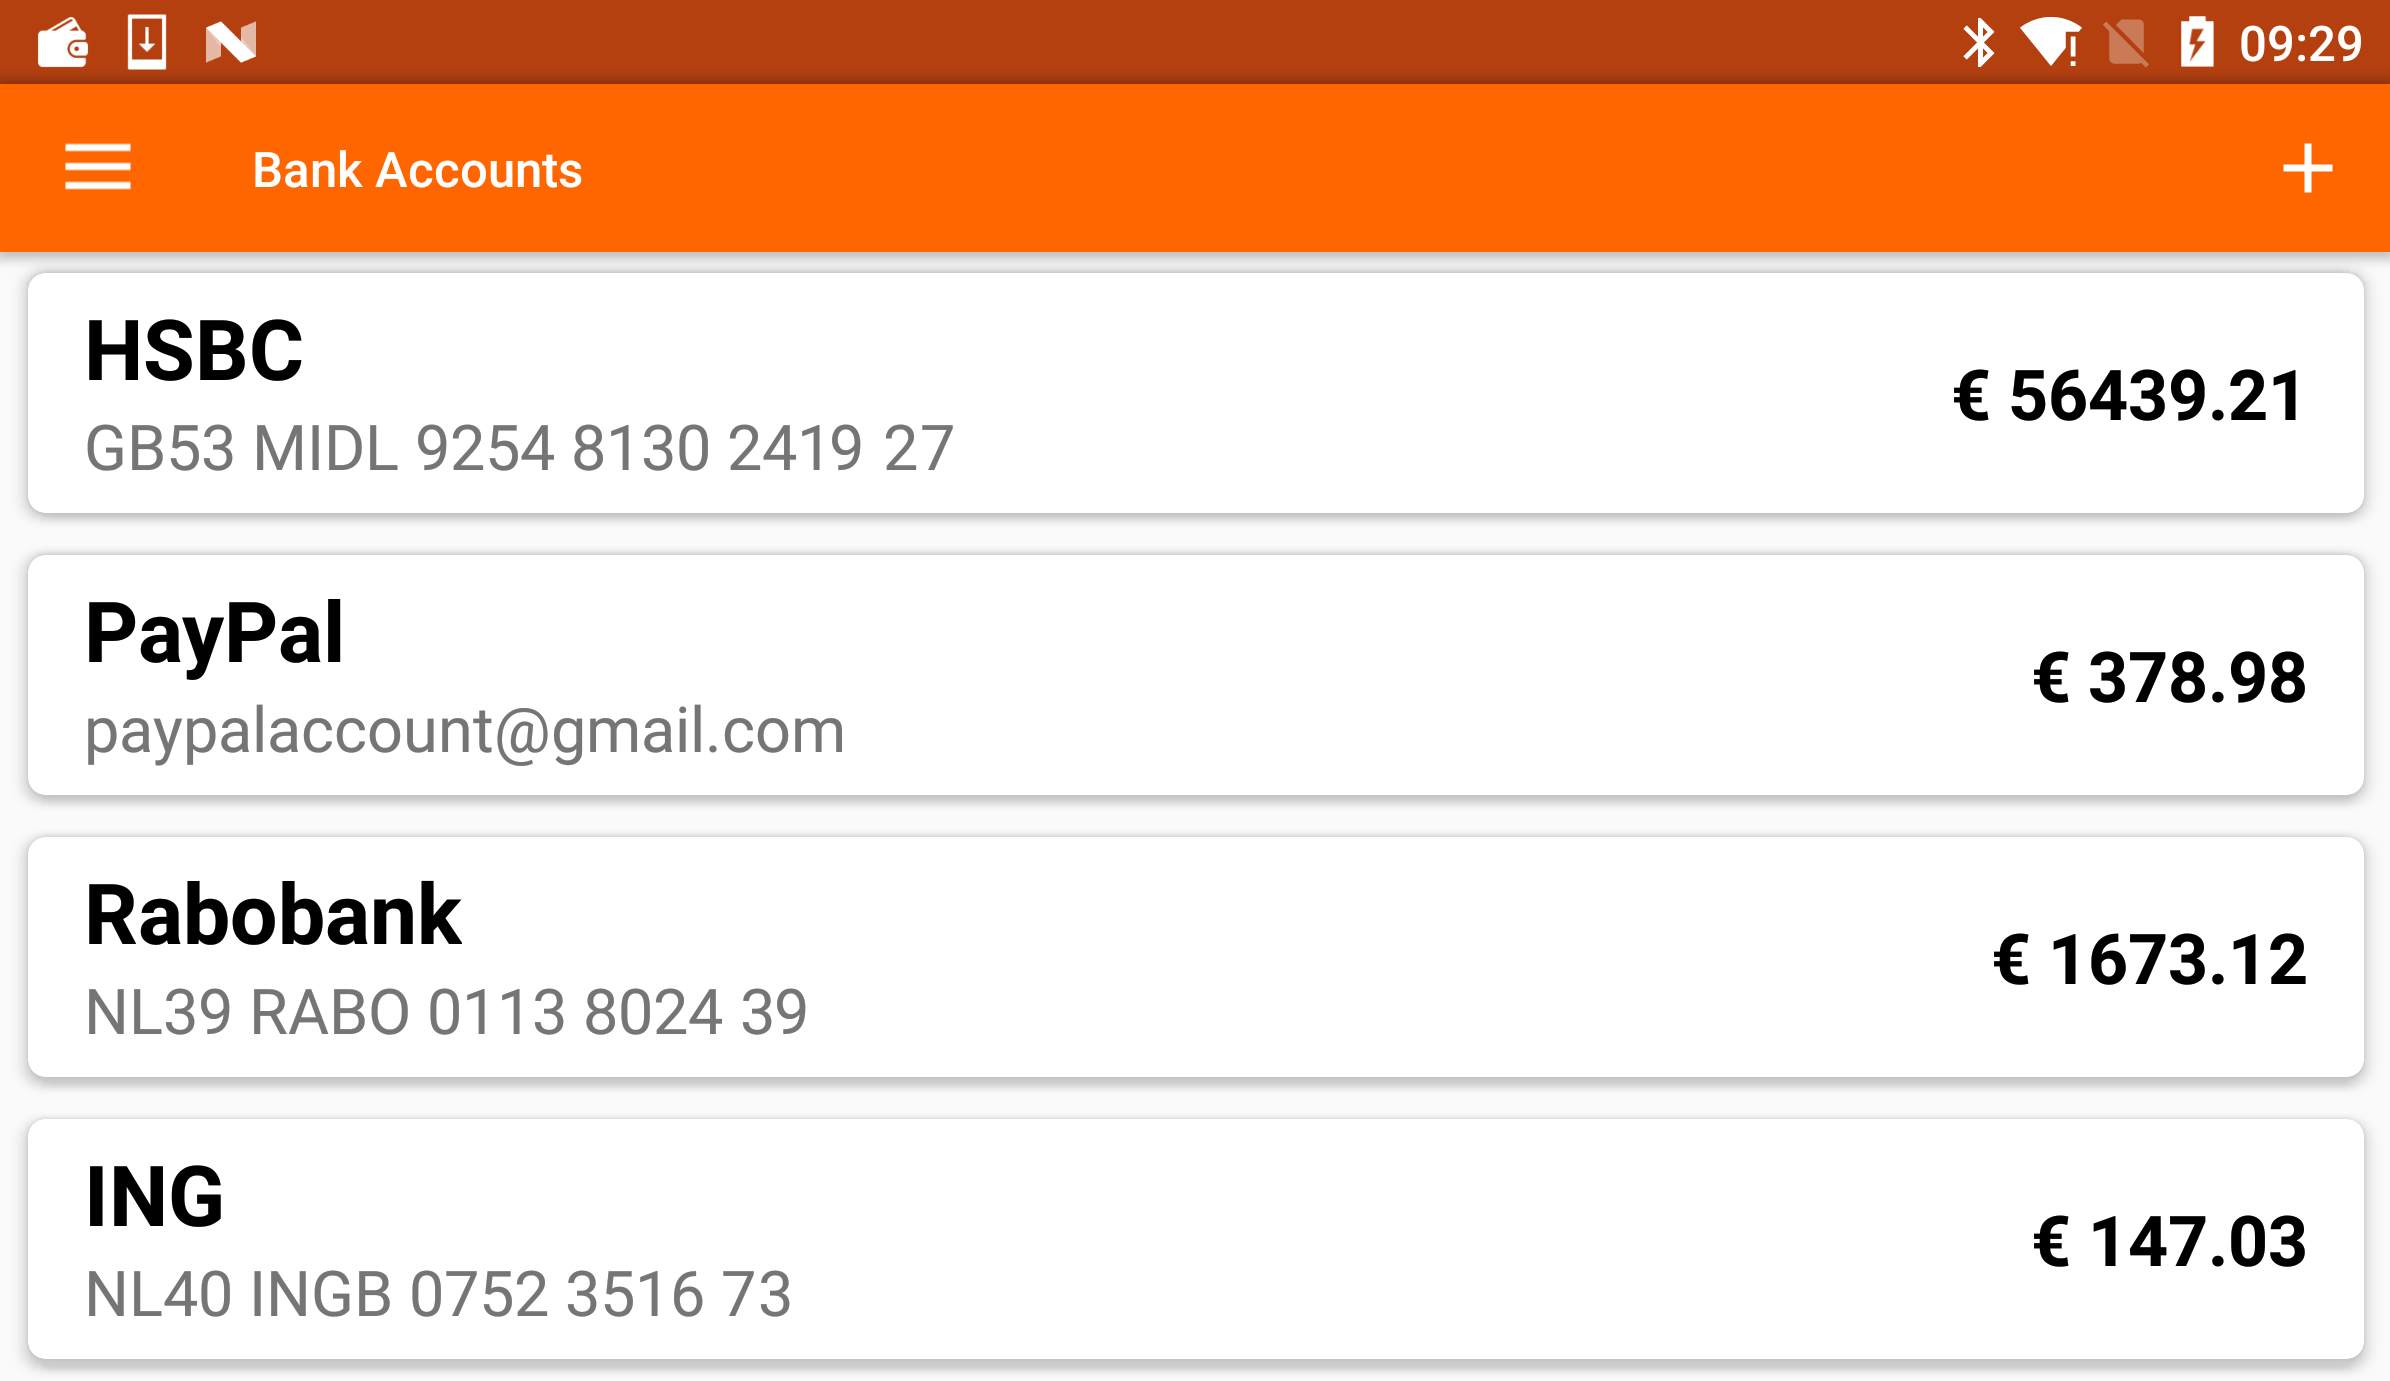
\includegraphics[width=.8\linewidth]{iom/assets/android}
	\caption{Our Android application to interface with different banks and to route money in real-time.}
	\label{fig:android_app}
\end{figure}

\section{Our Money Routing Mechanism}
% We provide the first alternative for trust provided by banks.
% We offer an intrastructure where any indivual can route money between bank accounts.
% Our first step is to provide sub-second money transfers and a basic trust system.
% We believe over time, this approach could be faster, cheaper and safer than the legacy banking system.

%Our work mixes existing bank accounts with blockchain technology.
Our mechanism to perform real-time payments is based on the observation that in-house payments are settled fast.
For the banks that we tested, intra-bank money transfers are settled within mere seconds (see Section \ref{sec:settlement_inhouse_experiment}).
Instead of using a central bank as settlement institution, we build a network of individuals that have bank accounts with multiple banks to perform settlement on a gross basis.
This works as follows: assume a Dutch buyer holding a Rabobank account, intends to pay a British merchant that holds a bank account with HSBC.
When this buyer initiate a payment with existing software to the merchant, then the funds can take several days to arrive in the bank account of the merchant.
However, when using an intermediary holding accounts both at Rabobank and HSBC, the buyer first sends the funds to the Rabobank account of this intermediary after which the buyer instructs the intermediary to forward the same amount of money from his HSBC account to the HSBC account of the merchant.

\begin{figure}[t]
	\centering
	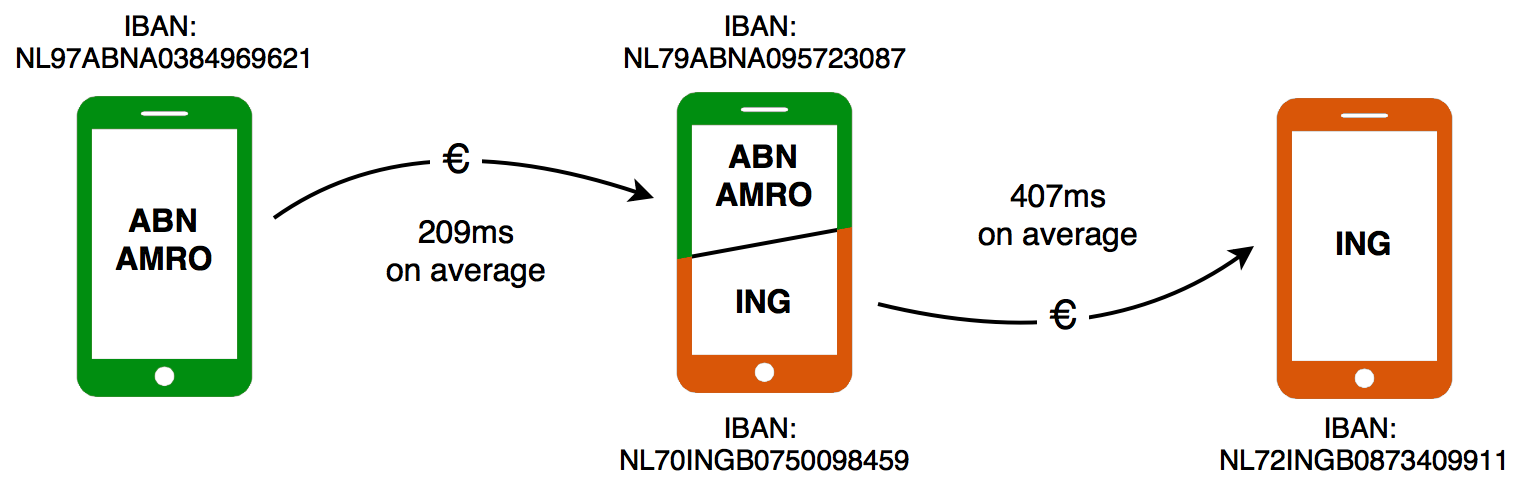
\includegraphics[width=\textwidth]{iom/assets/internet_of_money.png}
	\caption{The essence of the Internet-of-Money architecture: the smartphone in the middle acts as a money router using both ING and ABN AMRO bank accounts.}
	\label{fig:internet_of_money}
\end{figure}

Since this way of sending money only involves two in-house payments, the merchant receives the funds within a few seconds.
We call this process a \emph{fast payment}
We call the intermediary settling the transaction a \emph{money router}.
%The money transfer from buyer to merchant using money routers is called a \emph{fast payment}.
We use the terms \emph{initiator} and \emph{beneficiary} to indicate the initial sender and final receiver of a fast payment, respectively.
A fast payment can be facilitated by multiple routers to increase efficiency and availability.
%Depending on router availability, one might utilize multiple money routers for a single payment.
Note that fast payments lead to mutations in the account balances of the involved money routers.
This problem is addressed in Section \ref{sec:system_design}.
%This imbalance can be restored by a single payment by the intermediary at fixed time intervals, for instance, at midnight.

Fast payments have three major advantages for users.
First, it creates an open ecosystem for settlement activities, which benefits transparency and reduces the need for a central bank.
Second, inter-bank settlement durations are significantly decreased, from days to seconds. % when using others as financial intermediary.
Third, we reduce costs for inter-bank payments since no communication between banks is required, except when restoring balances (see Section \ref{sec:system_design}).
%We only rely on inter-bank payments when restoring balances between accounts of a money router.

Our system shares characteristics with services provided by Transferwise.
Transferwise is a currency exchange service to offer a cheaper alternative to established institutions when making international payments.
It routes payments not by transferring the sender's money directly to the recipient, but by redirecting them to the recipient of an equivalent transfer going in the opposite direction.
The essential idea is to convert international money transfers into a sequence of local transactions.
Their approach is comparable with our money router mechanism, as it also aims to reduce fees and improve efficiency of traditional payments.
However, international payments with Transferwise can still take a few days to complete, depending on the settlement duration of involved banks.

In the remainder of this work, we elaborate our trust model and technical specifications of money routing.
This includes an overlay network where any individual is able to quickly route money between bank accounts.
A screenshot of our built Android application is shown in Figure \ref{fig:android_app}.
The mobile application allows interfacing with different banks and the initiation of real-time payments using our overlay network.

%We implemented this idea and built an Android application, capable of communicating with different banks.
%A screenshot is presented in Figure \ref{fig:android_app}. 
%Finally, it is built upon existing infrastructure, reducing the barrier for adoption.

% We believe over time, this approach could be faster and cheaper for customers while providing a future-proof overlay, capable of replacing legacy banking systems.
% By building an open ecosystem, we aim to increase competition and efficiency of traditional payments.

%Essentially, Internet-of-Money is a two-sided, open market for clearing and settlement, operated by individuals acting as financial  intermediaries and others utilizing these.

%To elaborate our idea further, consider a transaction between Alice and Bob where Alice holds a bank account with Rabobank and Bob is a customer of ING.
%Further assume that there is an entity who owns bank accounts with Rabobank and ING, say Caroline.
%If Alice would send money directly to the bank account of Bob, settlement would take a considerable amount of time due to slow settlement cycles of the central bank.
%Instead, Alice first sends the money to the Rabobank account of Caroline and notifies her of the sent funds.
%We refer to Caroline as a \emph{money router}.
%Next, Caroline forwards the same amount of money from her ING account to the ING account of Bob.
%Note that this procedure only involves in-house payments and Bob receives the funds within seconds.

%After Caroline forwarded the received funds to the bank account of Bob, the distribution of balances on Caroline's accounts has changed.
%She is able to restore this balance by initiating transferring funds from her ING to her Rabobank account, essentially \enquote{recharging} her bank accounts.
%She can perform this transaction at any desired time.
%It is important to note that the capacity of a money router is limited by available balances on the accounts of a router.

%Throughout the remainder of this work, we will elaborate on trust estimation of money routers, fraud detection and discovery of eligible intermediaries.

\begin{figure*}[b]
	\centering
	\begin{subfigure}{.5\textwidth}
		\centering
		\captionsetup{width=.9\linewidth}
		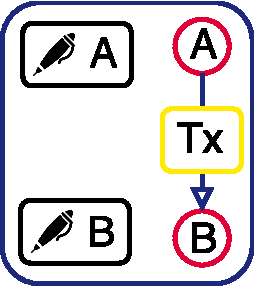
\includegraphics[width=.35\linewidth]{iom/assets/trustchain_tutorial_1}
		\caption{A transaction (\emph{Tx}) between two users ($ A $ and $ B $), with two digital signatures.}
		\label{fig:trustchain_tutorial_1}
	\end{subfigure}
	\begin{subfigure}{.5\textwidth}
		\centering
		\captionsetup{width=.9\linewidth}
		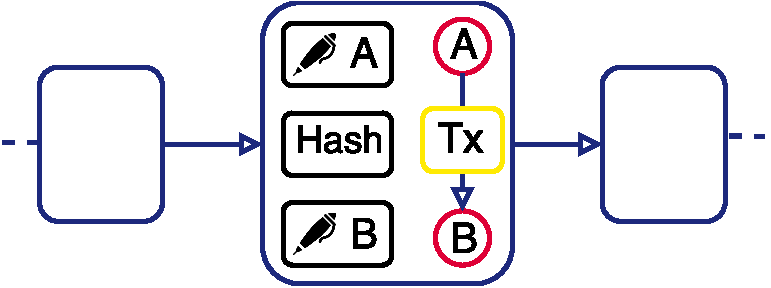
\includegraphics[width=\linewidth]{iom/assets/trustchain_tutorial_2}
		\caption{A blockchain of transactions. Each record in the chain points back to the previous one.}
		\label{fig:trustchain_tutorial_2}
	\end{subfigure}\vspace{0.3cm}%
	\begin{subfigure}{.5\textwidth}
		\centering
		\captionsetup{width=.9\linewidth}
		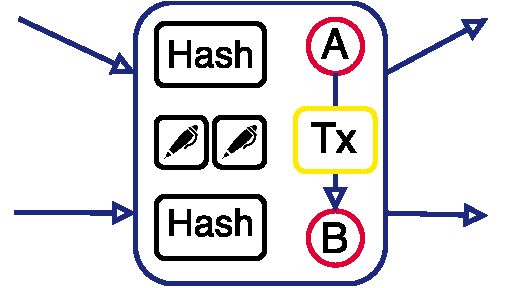
\includegraphics[width=.7\linewidth]{iom/assets/trustchain_tutorial_3}
		\caption{To increase security, each record also references a record in the chain of the other transaction participant.}
		\label{fig:trustchain_tutorial_3}
	\end{subfigure}
	\caption{Recording a transaction between two users $ A $ and $ B $ in TrustChain.}
	\label{fig:trustchain_tutorial}
\end{figure*}

\begin{figure}[b]
	\centering
	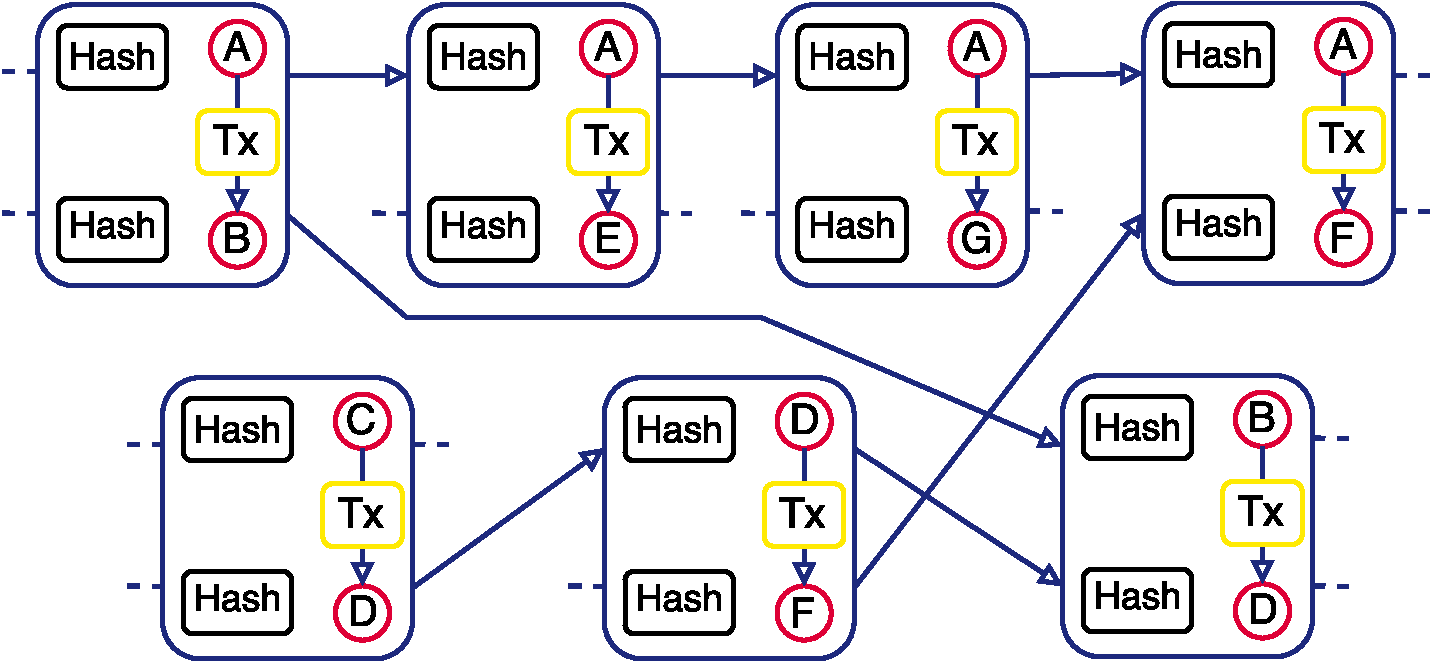
\includegraphics[width=.9\linewidth]{iom/assets/trustchain}
	\caption{The tamper-proof TrustChain data structure to record transactions.}
	\label{fig:trustchain}
\end{figure}

\section{Building Trust using Blockchain Constructs}
\label{sec:trust}
%We now present our blockchain-based trust model, used to determine trustworthiness of intermediaries and to exclude malicious nodes from the community.
We now explain our deployed, scalable blockchain fabric to gradually build trust between fast payment initiators and money routers: \emph{Trustchain}.
TrustChain is designed around transacting entities and is able to accurately capture interactions between users.
We have successfully explored usage of TrustChain for bandwidth accounting, attestations and decentralized trading in prior work~\cite{pouwelse2017laws}. % , and stores historical interactions.
%In Trustchain, every network participant operates his own chain of historical record.
%This is a fundamental difference with traditional blockchain solutions like Bitcoin or Ethereum where there is single ledger secured by the efforts of the network.
For an elaborate evaluation of TrustChain, we refer the reader to our published article~\cite{otte2017trustchain}.

Figure \ref{fig:trustchain_tutorial} illustrates how a transaction is recorded between two users on TrustChain.
Figure \ref{fig:trustchain_tutorial_1} shows a single transaction (\emph{Tx}).
Both parties sign the transaction with any cryptographically secure digital signature algorithm (our implementation uses ECDSA).
This makes participation irrefutable and acts as an agreement for the transaction specifications.
These digital signatures can efficiently be verified by others.
After signing, the transaction is committed to the local databases of both transacting users.

A natural way to order records in a database is to chain them together, ordered by creation time.
This is shown in Figure \ref{fig:trustchain_tutorial_2} where each record is extended with a pointer that points back to the prior record.
In particular, this pointer is a hash computed from the description of the prior record using any cryptographically secure hashing algorithm (our implementation uses SHA256).
Each record is equipped with a sequence number $ s \in \mathbb{Z} $ (the sequence number of the genesis record is 1).
This database organisation resembles a blockchain data structure.
While cryptocurrencies like Bitcoin and Ethereum operate on a global blockchain, TrustChain gives each user their own personal chain.

Outside for the user operating a chain, the structure shown in Figure \ref{fig:trustchain_tutorial_2} is void of any control.
Consequentially, a user is able to tamper with his historical transactions.
For instance, individuals are able to remove transactions that are not beneficial for their standing in the network.
After modification of a record, validity of the chain can simply be restored by recomputing all prior pointers.
To protect against local modifications, we extend each record with an additional pointer that points to the prior record in the chain of the transaction counterparty.
This ensures that each record has exactly two incoming and two outgoing pointers, as shown in Figure \ref{fig:trustchain_tutorial_3}.

When two users transact, their chains essentially become interleaved or \enquote{entangled}.
This property makes fraud impractical to hide since a counterparty is able to proof malicious activities by revealing his record of the disputed transaction.
%This reveals his perspective on the transaction.
When users initiate more transactions with others, they quickly become entangled in the network, leading to a directed acyclic graph (DAG) structure as shown in Figure \ref{fig:trustchain}.
This figure shows seven records, created by seven unique participants.
Users are able to collect records stored by others.
This ensures adequate replication of TrustChain records throughout the network.
%The TrustChain data structure is our core mechanism to build trust.

\subsubsection*{Recording Payments}
We use the TrustChain data structure to record money transfers between individuals.
%By constructing TrustChain records between individuals sending money to each other, we can keep track of.
Each payment and fast payment is assigned a unique identifier.
We define two different transaction types:
\begin{enumerate}
	\item \emph{commit}: This transaction is a public commitment by a money router to forward received funds.
	It is signed by the initiator of a fast payment and other money routers, prior to transferring any money. The transaction includes the identifier of a fast payment and account address of the money router that should forward funds.
	\item \emph{sent}: This transaction type is signed by two parties involved in an in-house payment and implies that money has been sent and received. This transaction includes the fast payment identifier and a boolean that is true if and only if the payment volume is above a threshold $ t $. 
\end{enumerate}
We deliberately choose to hide the exact payment volumes due to privacy considerations, at the cost of reduced information.
%We consider investigating the value of $ t $ outside the scope of this work.
%Initially, we fix this value to the median of payments made in the SWIFT system.

\subsubsection*{Detect and Punish Fraud}
The most challenging scenario occurs when a money router promises to forward money, but fails to do so.
Since TrustChain provides us with a public ledger, disputes can be detected between transacting entities.
Consider the situation when a router promised to forward money to Alice and claimed to have done so but Alice has not observed these funds (yet).
Other individuals are informed of this situation when they observe a \emph{commit} transaction, signed by both parties, and a \emph{sent} transaction that is only signed by the money router that didn't forward the funds yet.
As soon as such a dispute is detected, we do not consider this money router as intermediary for future fast payments until the dispute has been resolved.
Note that a dispute can also occur when a router is unable to forward money, due to downtime of involved banks or insufficient account balance.
%Distinguish between these situations could be made by relying on status reports by the involved banks.

In addition to the aforementioned scenario, a user can intentionally lie that he or she has not received funds from a money router. %, and slander a specific money router.
It is impossible to make statements about the status of a specific payment without access to both bank accounts involved in a payment.
To resolve disputes, we propose to use input from a dispute arbitrator in the form of an official, digitally signed statement.
The dispute arbitrator can be any company that is able to query bank accounts, for instance, the bank involved in a fast payment.
A statement provides the status of a fast payment with a specific identifier and should be published on the TrustChain ledger.
To discourage users from purposely creating disputes, the arbitrator should charge a small fee for publishing a statement, say \euro 0.10.
This fee should be covered by the party that made a false statement about money being sent or received.
Note that dispute arbitration enables a new business model for banks.
%Note that this enables a new business model for banks.
%To resolve a dispute, we propose input from the involved financial service providers is required in the form of an official, signed bank statement.


% Bank statement

%This type of fraud can either occur intentionally or unintentionally, due to technical issues in the banking system.

\subsubsection*{Quantifying Trustworthiness}
\label{sec:estimate_trust}
We now discuss a mechanism to quantify trustworthiness of honest money routers.
%While fraud detection is an essential primitive, we also require a mechanism to quantity trustworthiness of honest routers.
Our proposed solution is based on past settlement services provided by money routers.
%We now describe a reputation mechanism to estimate trustworthiness scores to money routers, based on settlement services provided in the past.
We define a credit network $ G $ that models how much money a participant trusts to another individual.
The graph is built using collected, dual-signed TrustChain transactions from others.
Let $ T_{a,b,R} $ indicate a successful money transfer from user $ a $ to $ b $ using the routers in the set $ R $. % (indicated by \emph{commit}/\emph{sent} transactions).
Let $ (a, b, w) $ indicates a directed edge in $ G $ from user $ a $ to $ b $ with weight $ w $.
Now, each identity in our TrustChain network is modelled as a node in $ G $.
For each $ T_{a,b,R} $ and each router $ r \in R $, we create two directed edges: $ (a, r, w) $ and $ (b, r, w) $ where $ w = min(0.01, t) $ (the minimum monetary value we trust to someone is \euro 0.01).
These edges represent trust in routers that have forwarded incoming money in the past.

To determine trust scores, we use an algorithm which has been studied extensively in related work, personalised PageRank~\cite{page1999pagerank}. %each user executes the personalized PageRank algorithm on $ G $, which assigns a score between 0 and 1 to each node in $ G $~\cite{page1999pagerank}.
The algorithm assigns a score between 0 and 1 to each node in $ G $.
These scores are used to pick intermediaries for money forwarding (see Section \ref{sec:system_design}).
We consider the node in $ G $ that performs the computation as trusted source.
Using a reputation algorithm based on random walks is attractive due to its high scalability and low computational complexity.
However, one might consider using a reputation algorithm based on maximum network flow to compute trust scores.
In particular, we believe the Bazaar algorithm is suitable for this use case and provides additional security at the cost of increased computational requirements~\cite{post2011bazaar}.

\subsubsection*{Preventing the Sybil Attack}
%Our current model allows manifestation of a Sybil Attack where an attacker operates multiple entities that use the same bank account for money routing.
We propose a mechanism called \emph{router validation} to ensure that a specific bank account can only be operated by a single money router.
The effectiveness of this method comes from the difficult and costly process of opening many accounts with different banks internationally. %, in particular internationally.
This addresses the challenging Sybil Attack, where an attacker operates multiple entities that use the same bank account for money routing.
A router first registers a bank account by sending \euro 0.01 to a trusted third party (TPP), for instance, a bank.
The digital identity of TPPs are publicly available.
TPPs sign and store a so-called \emph{verify} transaction on TrustChain together with a money router when the payment is observed.
This transaction uniquely connects a bank account to a money router.
Routers reusing accounts across multiple identities can be identified by querying TrustChain records.

\section{System Design of Internet-of-Money}
\label{sec:system_design}
We expand upon fast payments and our trust model by designing a novel overlay network named \emph{Internet-of-Money}.
It operates on top of existing inter-bank payment systems, similar to how The Internet was built on top of the legacy telephone infrastructure.

\subsubsection*{The Money API}
Except for the German FinTS payment protocol, there are no open standards yet for online banking.
European legislation called PSD2 is forcing all EU banks to create open interfaces (APIs)~\cite{cortet2016psd2}.
We created one of the first open implementations capable of communicating with numerous banks. % online banking 
%Based on existing networking protocols of banks, we created an unpermissioned, unified interface for online banking.
%This results in each company building applications around their own requirements, resulting in a large number of non-compatible communication protocols.
%We combined the proprietary protocols of banks.
%As a first step towards sub-second money transfers, we combine the proprietary protocols of banks.
We combined banks in the Netherlands (Rabobank, ING and ABN Amro), the British bank HSBC and the Luxembourg payment provider PayPal~\cite{doe2015vulnerability}\cite{awesome2015vulnerability}.
We devised a single API to communicate with all these banks, called \emph{The Money API}.
The Money API provides primitives to login, fetch account balance, query mutations, initiate payments to other accounts and register devices.
This library is designed to be extendible and we have partial support for banks in Italy, Greece, Sri Lanka, Turkey and Germany.
Our open source\footnote{The Money API source code:\\http://www.ds.ewi.tudelft.nl/fileadmin/pds/homepages/vos/\\iom/internet\_of\_money.zip} library is currently being tested.

%We are currently unable to publicly release the implementation of our unified interface yet due to open legal considerations.
%Ongoing collaboration with business partners focusses on exploring legal considerations of the Money API.

\subsubsection*{Money Routers}
Each money router must offer settlement services with at least two different bank accounts.
Having many money routers in the network directly benefits availability and load balancing.
A study conducted by NGData indicated that 37.7\% of the respondents held accounts at different banks and are able to act as settlement intermediary for money transfers~\cite{ngdata2014consumer}.
To create incentives for users to operate a money router, we include transaction fees.
%To incentivize users to operate a money router, Internet-of-Money allows specification of transaction fees that users have to pay to make fast payments.
Transaction fees can be either fixed, defaulting to \euro 0.01, or a percentage of a fast payment volume.
These fees are necessary to cover costs enforced by banks when initiating cross-border payments or when using business accounts to route money.
In addition, users can specify a minimum account balance to avoid taking costs when their balance becomes negative.
In the remainder of this work, we assume transaction fees are fixed.
We also consider an analysis of monetary incentives out of scope and not fundamental for the prototype evaluated in this work.

Note that our design also allows the role of money router to be fulfilled by a single trusted third party or by a few selected trustworthy entities (i.e. financial institutions).
A more centralized architecture would mitigate some of the trust and security issues that arise from full decentralization.
However, we consider open enrollment (the opportunity for any user to act as a money router) a cardinal property of our system.
% Huidige users kunnen nu geen money routers worden

\subsubsection*{Router Discovery}
\label{sec:peer_discovery}
%For discovery of available money routers in the network, we do not rely on a centralized service.
We designed a gossip protocol for discovery of available money routers, based on utility.
Like all our proposed infrastructure, it does not depend on any server, company, or other central entity.
%Discovery of available money routers in the network relies on a decentralized gossiping mechanism.
%Instead, router availability is disseminated with a decentralized gossiping mechanism.
%We devised a protocol to gossip routers based on utility provided by each router.
If Alice wishes to discover a new router, she asks one of her known peers, say Bob, to introduce a router to her.
Now, Bob tries to introduce a router to Alice through which she can route money. %an entity Trudy when Alice is able to route money using the bank accounts owned by Trudy.
In general, the algorithm prioritizes routers that provide the most benefit to Alice.
%Next, we prioritize routers with a higher variety of bank accounts since they are able to provide additional services.
If Bob has no router in his set of known peers that are able to provide new services to Alice, he will introduce a random router to Alice.
Repeating this gossiping protocol quickly converges to a network with connections between individuals able to provide routing services for each other.
An evaluation of this mechanism is given in Section \ref{sec:router_discovery_evaluation}.

\subsubsection*{Building a Money Circuit}
Prior to transferring money, an initiator of a fast payment starts by selecting eligible routers that are capable of handling the upcoming fast payment.
We define a \emph{money circuit} as the set of peers that are involved in a fast payment.
This set contains at least one initiator and one beneficiary, and optionally one or more money routers.
A money circuit that contains $ n $ money routers, is called a $n$-hop circuit.
Building a money circuit proceeds in a depth-first manner and starts with the initiator selecting a router, say $ r $, that is capable of routing money to another account.
Next, the initiator sends an \emph{extend} message to $ r $ which contains the payment volume and the destination bank account of the fast payment.
$ r $ responds with a boolean that indicates whether $ r $ has sufficient funds to handle the transfer.
The response also includes a list of routers that are able to extend the money circuit, and the transaction fee charged by $ r $.
If $ r $ is able to handle the transfer, the initiator picks a router to extend the circuit with and sends an \emph{extend} message again.
These routers are picked based on trustworthiness scores.
This process repeats until the initiator built a money circuit that can handle the fast payment. % to the account of the beneficiary.
Users are able to change the maximum number of routers in a circuit, which defaults to 3.
%Once a circuit is established, the initiator queries transaction fees of each router.
%The sum of these fees give the total transaction fees for a specific fast payment.

%When assigning a trustworthiness score, we only consider historical behaviour of a money router.
The trust model discussed in Section \ref{sec:trust} is based purely on past transactions.
It is useful to consider other properties when picking eligible money routers, such as transaction fees, availability, reliability or network latency. 
Depending on the situation, one might favour low network latency or competitive transaction fees over trustworthiness.

%However, when selecting an eligible money router for a fast payment, it is helpful 

\subsubsection*{Transferring Money}
We now elaborate the process of transferring money over a $ n $-hop circuit.
%First, an initiator generates a random identifier, used to track fast payments going over a money circuit.
If $ n = 0 $, money is sent directly to the beneficiary using exactly one in-house payment and no money routers.
A single \emph{sent} transaction is created between the fast payment initiator and beneficiary.

When a money circuit involves one or more money routers ($ n \geq 1 $), the fast payment is facilitated by intermediaries.
Let $ r_i $ indicate the $ i $-th router in the circuit ($ r_1 $ represents the first router).
The initiator starts by sending a message to $ r_1 $, containing the payment volume and all subsequent routers involved in the money circuit, including the final beneficiary of the fast payment.
Next, the initiator initiates a \emph{commit} transaction with $ r_1 $ and sends the money.
$ r_1 $ now starts to poll for the money and finally constructs a \emph{sent} transaction when funds are observed.
%Recall that one \emph{commit} and one \emph{sent} record are created for each payment between two bank accounts.
%Now, $ r_1 $ creates a \emph{commit} record with $ r_2 $, initiates a payment to the bank account of $ r_2 $ and constructs a \emph{sent} record with $ r_2 $.
$ r_1 $ forwards the funds to the next router or the beneficiary and this process repeats until the money arrives in the bank account of the beneficiary.
The final transfer to the beneficiary does only result in a \emph{sent} transaction.
Thus, a fast payment with $ n $ intermediaries results in $ 2n+1 $ new records.

%first, the initiator construct a \emph{commit} record with $ R_1 $.
%Next, the initiator transfers the funds (including the sum of transaction fees) to $ R_1 $ and they construct a \emph{sent} record.
%This process repeats by the initiator creating a \emph{commit} record with $ R_2 $, sending the funds to this router and constructing a \emph{sent} record.
%By repeating this process, one is able to transfer money using multiple intermediary routers to any destination account.
%Note that this procedure only relies on in-house payments that settle relatively fast.

\subsubsection*{Risk Mitigation}
In addition to our trust model, we propose two risk mitigation techniques to reduce counterparty risk when using money routers:
\begin{enumerate}
	\item \emph{Incremental settlement}: A key risk mitigation technique is to avoid making a single, large payment at once. Instead, a payment is divided into $ n $ smaller inter-bank payments. While this increases duration of a fast payment by a factor $ n $, it significantly reduces risk and incentives for intermediaries to compromise money. We believe that reduced risk for some increased latency is a desirable trade-off in Internet-of-Money.
	\item \emph{Multi-flow payments}: We uniformly divide a fast payment amongst multiple, distinct money circuits. This results in smaller payments through intermediaries and less value at stake. With multi-flow payments, the end-to-end latency of a payment is determined by the slowest money circuit.
\end{enumerate}
While these individual strategies are viable to mitigate counterparty risk, combining them results in a significant reduction of the value at stake, at the cost of additional latency when using incremental settlement and communication overhead.
We evaluate the effectiveness of these strategies in Section \ref{sec:fraud_experiment}.

\subsubsection*{Router Recharging}
Since funds arrive in one account and leave another, money routers might become unable to route additional funds at one point in time.
This can be addressed by handling fast payments going in the opposite direction, which restores account balances.
However, initiation of these fast payments is outside the control of money routers.
Balances can also be restored by initiating a payment from the account with excessive balance to the other bank account.
Since this involves an inter-bank payment, settlement might be slow and in turn, this negatively impacts router availability.

This problem is also recognized in off-chain payment networks that are using channels between users with limited capacity.
Revive is a mechanism for rebalancing payment channels and avoids the need for (often expensive) transactions on a blockchain to recreate the channel~\cite{khalil2017revive}.
Alternatively, this issue can be addressed by the route discovery mechanism where routing decisions aim to minimize the amount of rebalancing required while maximizing user profits.

For our mechanism we envision an infrastructure where routers help each other to restore balances, effectively creating a two-sided market with capacity supply and demand.
For instance, a router can offer PayPal capacity in return for HSBC funds.
Rebalancing payments are handled by the Internet-of-Money mechanism.
While this is an efficient method to restore balances, only requiring in-house payments, we consider the design and implementation of such a mechanism as future work.

%We should realise that this approach is susceptible to errors which might lead to money not being transferred over a money circuit.
%This includes faults in our overlay, downtime of the financial service providers or insufficient funds by an individual to forward money.
%This highly motivates the requirement for a fault-tolerance mechanism.
%We address this issue by introducing a rollback operation, that is automatically initiated soon as a router is unable to forward money to the next router, for any of the reasons previously mentioned.
%During a rollback, a router automatically returns the money to the payment initiator and sends a message informing the initiator about the rollback\myworries{nog meer om fault-tolerance te garanderen?}.

%\subsubsection*{Router Validation}
\label{sec:switch_validation}
%During the router discovery mechanism, routers are able to claim that they own bank accounts that are actually not under their control.
%This opens possibilities for a Sybil Attack where malicious routers can create numerous fake identities and share access to a specific bank account to provide settlement services as intermediary.
%Additionally, when an identity does not forward received funds, he or she can simply create a new identity and operate under that.

%We address these attacks by proposing a mechanism called \emph{router validation} which uniquely links a digital identity to a bank account.
%In particular, it ensures that each bank account can only be operated by a single digital identity.
%The rationale of this mechanism is based on the fact that it takes some effort to open new bank accounts, in particular in countries foreign to a user.
%Switch validation is performed by trusted third parties (TPPs) that operate in the network.
%These validators publish their digital identity online and are able to handle account validation requests.

%Various financial institutions have a requirement for bank account validation when operating in their environment.
%This is often part of the Know Your Customer (KYC) regulation that aims to prevent such institutions from participating in illegal money laundering activities.
%Validation often proceeds by the customer being validated transferring a small amount of money to a specified bank account, sometimes with a specific payment description.
%Duration of this validation is limited by settlement cycles of the financial intermediaries and often takes multiple business days to complete.

%Duration of our validation mechanism takes mere seconds.
%It proceeds as follows: first, the user that wishes to validate a specific bank account, connects to one of the trusted validators and queries a challenge, which is simply a short random string.
%Next, the user performs a payment to the bank account of the validator where the challenge is embedded in the description of the payment and informs the validator about the payment (we assume the validator opened accounts with all supported banks).
%When the validator receives the funds, which should only take a few seconds since it considers an in-house payment, it compares the payment description \emph{for an exact match} with the required challenge and sends a verification response to the user being validated.
%This prevents an attack where a user use money routers to validate ownership of an account.
%When validation succeeds, the account address is linked to a specific public key by sign and this information is broadcast in the network by the validator.
%This allows network participants to query bank account validity of entities in the network.

\section{Experiments and Evaluation}
We now evaluate the performance of money routers, speed of router discovery within Internet-of-Money and the effectiveness of our trust model.

\subsection{Performance of Money Routing}
This section concentrates on the performance of fast payments using money routers.
All these experiments are conducted with real bank accounts and real money.

\begin{figure}[t]
	\centering
	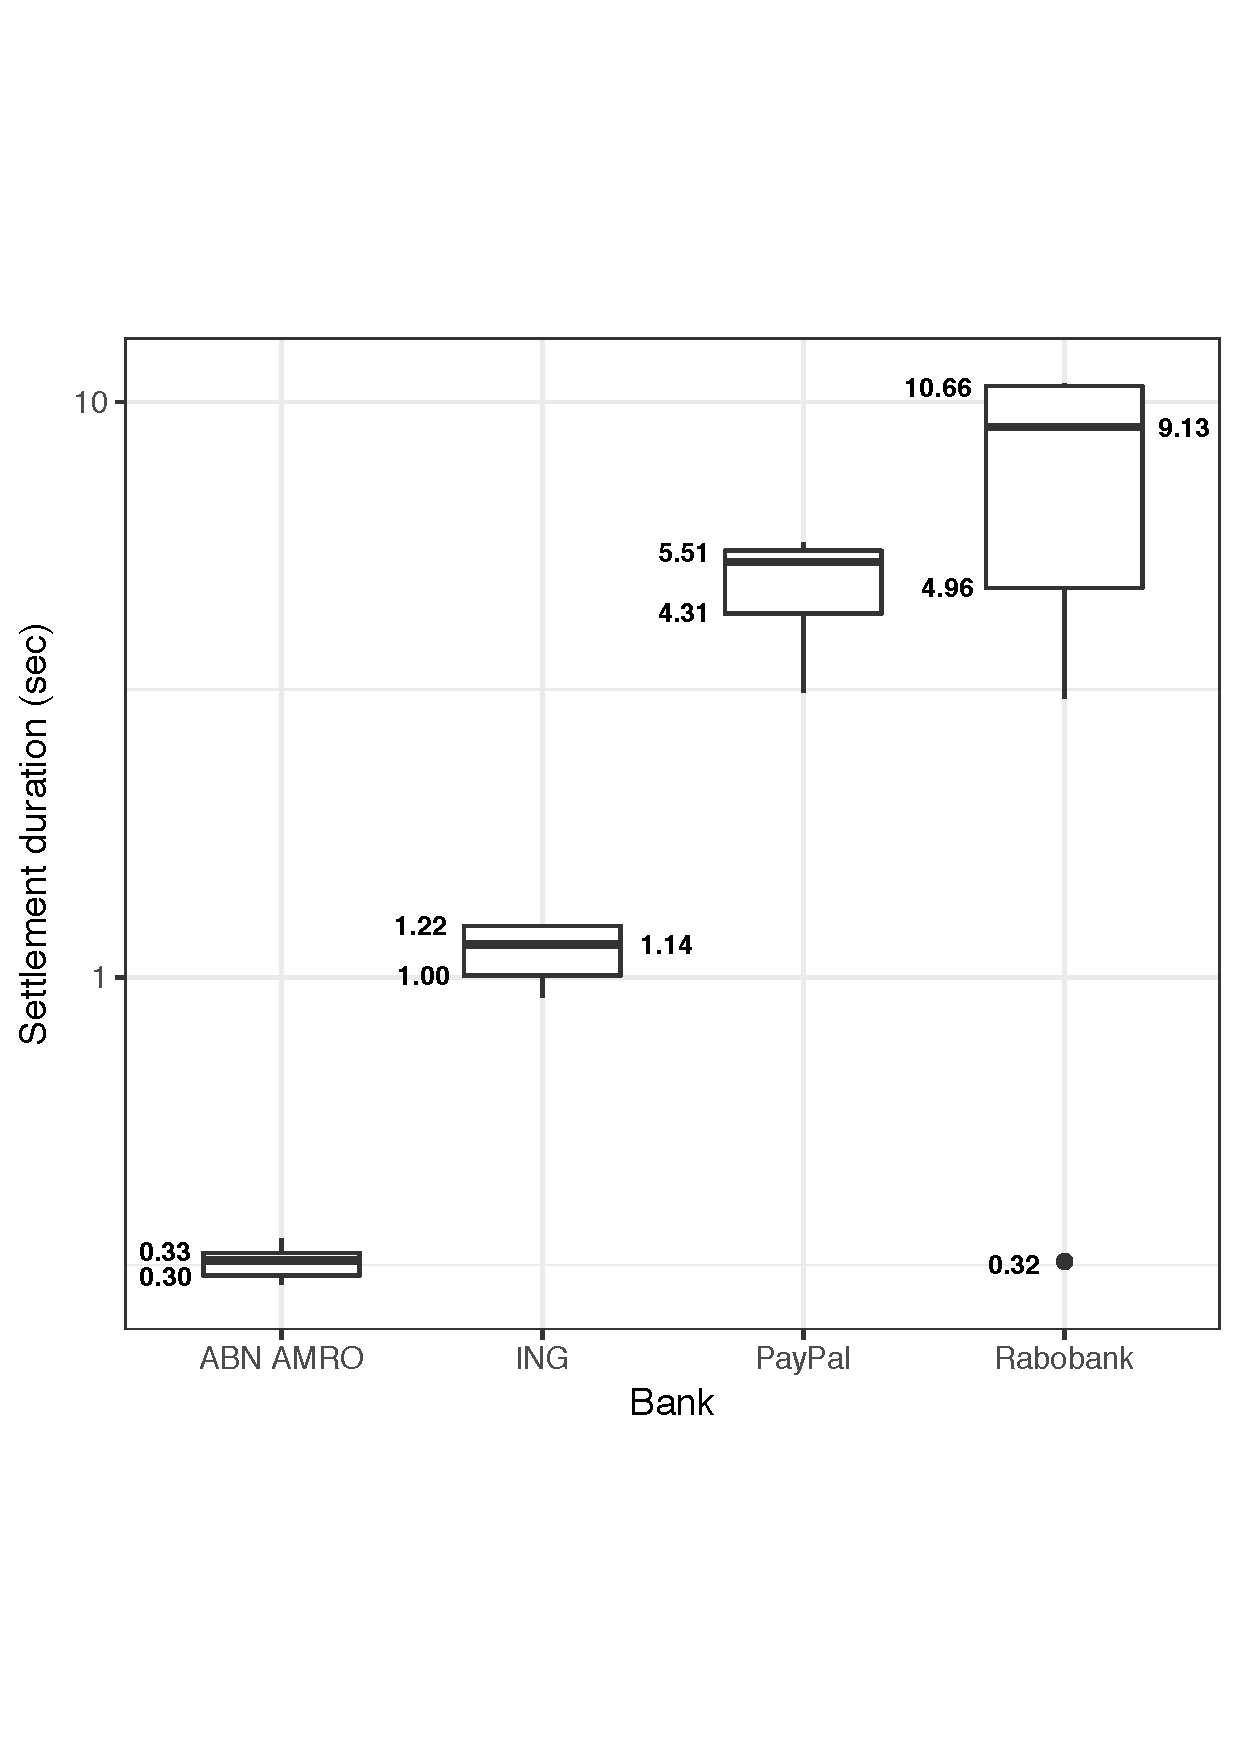
\includegraphics[width=.7\linewidth]{iom/assets/intrabank_annotated}
	\caption{Settlement durations of in-house payments for four supported banks.}
	\label{fig:intrabank_speed}
\end{figure}

\subsubsection*{Settlement duration of in-house payments}
\label{sec:settlement_inhouse_experiment}
%We determine the settlement duration of in-house payments. %performed within the same bank.
To determine settlement duration of in-house payments for each bank, we send \euro 0.01 ten times between two accounts with different holders, within the same bank.
By adding a unique identifier to the description field of a payment, we are able to track payments and accurately measure settlement times.
The experiment is executed with two clients on two different computers, with a polling interval of 500 milliseconds, to avoid hammering the bank servers.
Polling starts when the payment request has been finished by the sending party.
The results are shown in Figure \ref{fig:intrabank_speed}, with a non-linear vertical axis.
Only one bank, ABN AMRO, has sub-second settlement times with an average duration of 320 milliseconds.
ING is slower with 1109 milliseconds on average.
PayPal and Rabobank show settlement durations that are an order of magnitude slower, averaging to 4.82 and 7.61 seconds respectively.
When performing measurements for the Rabobank, we observed a notable outlier with a settlement time of 320 milliseconds.
This observation can be explained if we assume that similar internal payments might be handled in different ways by the Rabobank.
This experiment demonstrates that in-house payments are usually settled within seconds.
%An interesting observation is that Rabobank payments show a relative high variance in settlement duration, with a notable outlier of 320 milliseconds.

\begin{figure*}[t]
	\centering
	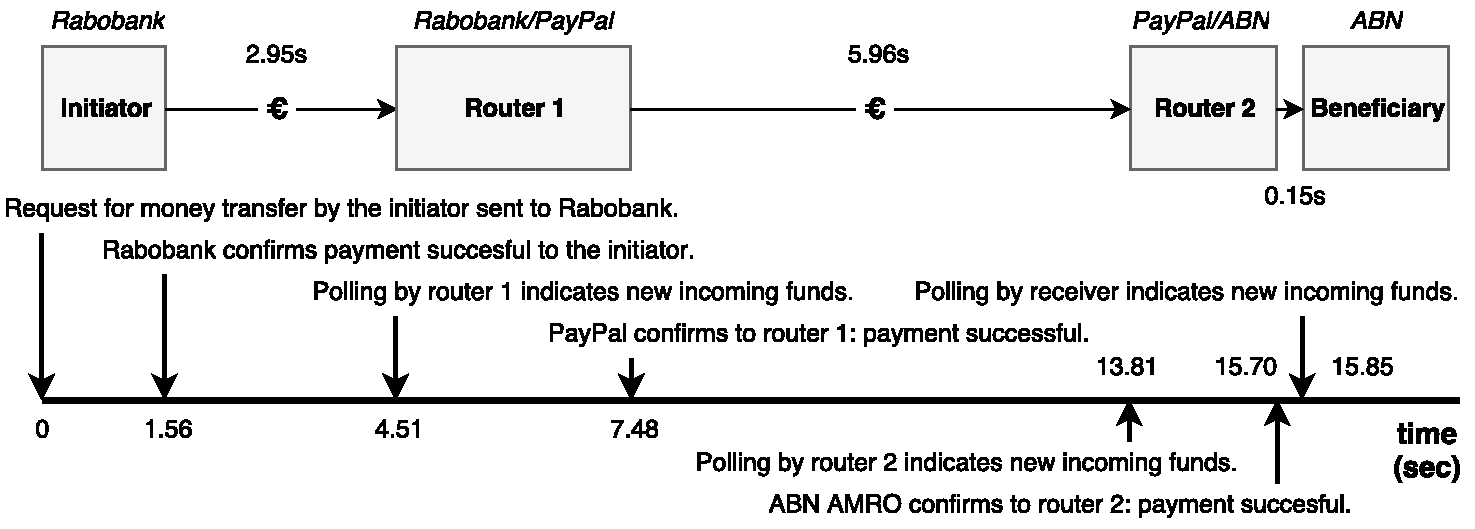
\includegraphics[width=\linewidth]{iom/assets/speedball}
	\caption{Timeline of an international fast payment from Rabobank to ABN AMRO, using two money routers.}
	\label{fig:speedball_experiment}
\end{figure*}

\subsubsection*{International Real-time Money Routing}
Next, we focus on the performance of an international fast payment and measure the duration of a money transfer from Rabobank to ABN AMRO, using two money routers.
This experiment aims to show the viability and speed of Internet-of-Money.
Figure \ref{fig:speedball_experiment} shows the experimental setup and timeline of our experiment.

First, an initiator sends funds from his or her Rabobank account to the first router (holding an account at Rabobank and PayPal), and informs it about the sent funds.
Next, the first router starts polling for incoming funds, with an interval of 500 milliseconds.
When the first router observes the funds, it forwards them to the second router (holding an account at PayPal and ABN AMRO) and informs this router.
When the second router observes the funds, it forwards the money from it's ABN AMRO account to the ABN AMRO account of the beneficiary.
In total, three in-house payments are made, with six different bank accounts.
%Unfortunately, we were unable to include ING accounts in this experiment since they were blocked shortly after conducting the previous experiment.

From Figure \ref{fig:speedball_experiment}, we conclude that it takes 15.85 seconds in total for money to arrive in the bank account of a beneficiary when using two intermediate routers.
A significant amount of time is spent on waiting for the funds to arrive in the PayPal account of the second router, around 6 seconds or 38\% of the total duration.
The average time to perform a payment is 2.14 seconds and initiation of payments take 41\% of the total duration.
The average time that a transaction is in transit is 3.02 seconds.
%40.5\% of the total time is spent on requests to perform payments.
The total time to perform a fast payment is heavily influenced by the type and number of intermediate routers.
This experiment demonstrates that Internet-of-Money is capable of real-time money routing to other banks.

\subsection{Overlay Evaluation}
The purpose of the following experiments is to quantify the performance of our money router overlay.
This includes an evaluation of our trust model and effectiveness of fraud detection.
We implemented our trust model and Internet-of-Money overlay network in the Python programming language.
Our implementation is built upon the Dispersy framework, providing primitives for peer discovery, decentralized communication and secure messaging~\cite{zeilemaker2013dispersy}.
%We evaluate our trust model and overlay using a real-world emulation, with a particular focus on router discovery and fraud detection.

\subsubsection*{Experimental Setup}
The following real-world emulations are executed on the DAS-5 supercomputer, using 50 instances per node~\cite{bal2016medium}.
We deploy our experiment using the Gumby framework and we create a scenario file where we schedule actions at specific times.
All code used during these experiments is open source\footnote{https://github.com/devos50/gumby/tree/iom\_experiment}.
Due to the limited number of accounts we own and to avoid a large load on the banking infrastructure, simulated accounts are used during this experiment.
We assume a total of five different banks and devised a basic RESTful banking server that handles account creation, payments, balance queries and mutation requests.
Distribution of bank accounts amongst users follows the data as published in the NGData customer banking survey (we assume that every user owns at least one bank account)~\cite{ngdata2014consumer}.

\begin{figure}[!t]
	\centering
	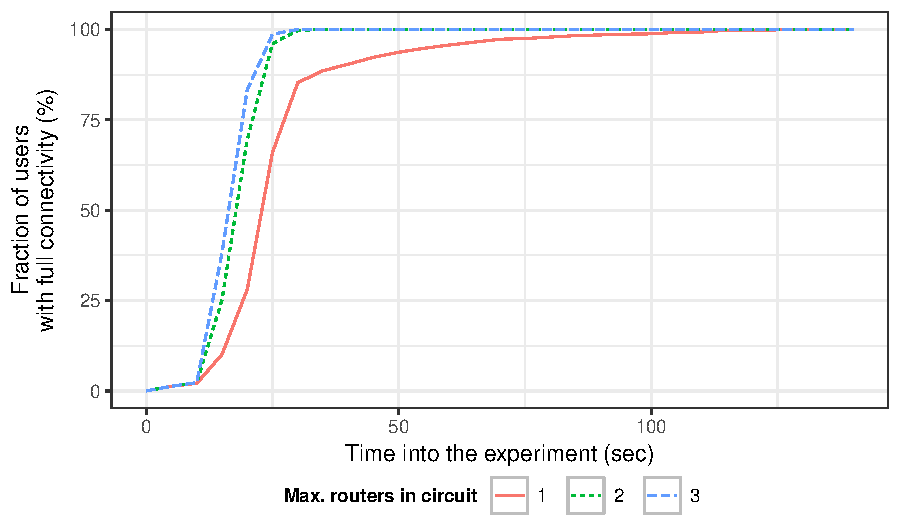
\includegraphics[width=.8\linewidth]{iom/assets/router_discovery_times}
	\caption{Performance of router discovery under a varying number of maximum hops in a money circuit.}
	\label{fig:router_discovery_times}
\end{figure}

\subsubsection*{Router Discovery}
\label{sec:router_discovery_evaluation}
We evaluate the efficiency of the router discovery protocol discussed in Section \ref{sec:peer_discovery}.
%We consider quick bootstrapping in the network important since fast payment initiators might not always be online.
During the experiment, we record the connected peers for each user at a fixed interval (every 5 seconds).
We determine whether this user is capable of transferring money to all five different bank accounts, using at most one, two and three intermediate money routers respectively.
%After starting the experiment, we log the connected peers for each user in the network every five seconds and determine whether this user is capable of transferring money to all five different bank accounts, using at most one, two and three intermediate money routers respectively.

Figure \ref{fig:router_discovery_times} shows the performance of router discovery in the Internet-of-Money overlay.
The horizontal axis denotes the time into the experiment.
The vertical axis indicates the percentage of users that are able to make fast payment to all five banks, or are fully connected.
We vary the maximum number of routers in a money circuit.
As expected, it takes longer before users are able to build circuits to all other banks using only one router, compared to three routers.
However, the differences are marginal.
In general, router discovery happens fast: 50\% of all users are able to make fast payments to all banks within 25 seconds after the experiment starts.
40 seconds into the experiment, this percentage increased to 90\%.
Note that it takes longer before \emph{all} users are fully connected using at most one intermediate router: 140 seconds.

\begin{figure}[!t]
	\centering
	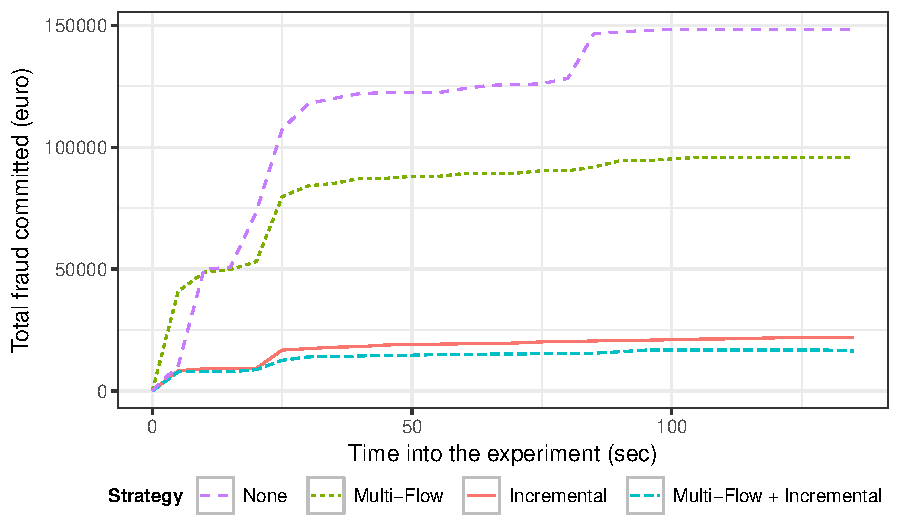
\includegraphics[width=.8\linewidth]{iom/assets/fraud_experiment}
	\caption{The effectiveness of fraud prevention, with different risk mitigation strategies.}
	\label{fig:fraud_experiment}
\end{figure}

\subsubsection*{Fraud Detection}
\label{sec:fraud_experiment}
Our final experiment focusses on the effectiveness of fraud detection (see Section \ref{sec:trust}). %, in particular, our mechanism to prevent fraud.
To this end, we emulated 200 users with one or more bank accounts.
Every five seconds, each user with a single account initiates a fast payment to another entity that has exactly one account of a different type.
This forces a money router in the established circuits.
The volume of each fast payment is picked from a uniform random distribution between \euro 0.01 and \euro 1000.
We challenge ourselves and assume that every user with at least two different bank accounts is malicious and has a 50\% probability of committing fraud and not forwarding received funds during a fast payment.
To improve router availability, we connect all peers together before the experiment starts.
In total, we schedule payments which volume sums to \euro 1,251,848.35.

The results are shown in Figure \ref{fig:fraud_experiment}.
The horizontal axis denotes the time into the experiment in seconds, after users start performing fast payments to each other.
The vertical axis shows the total amount of committed fraud in Euro.
We run the experiment four times with different risk mitigation strategies, namely incremental settlement (we split each fast payment in five equal parts) and/or multi-flow payments.
The figure hints that the amount of fraud is capped and that malicious routers are successfully excluded from money circuits.
Without any risk migration strategy, malicious routers are able to steal \euro 1,544 on average during the whole experiment, indicating that fraudulent routers are able to commit fraud multiple times.
This can be addressed to the fact that they are included in multiple money circuits roughly at the same time. 
If we consider risk mitigation strategies, we see that the combination of multi-flow payments and incremental settlement leads to the lowest amount of fraud possible, on average \euro 174.
Using exclusively incremental settlement leads to a slightly higher amount of fraud.

\section{Discussion}
\label{sec:discussion}

We now discuss this research from various perspectives.

\subsubsection*{Legal}
The idea of directly sharing funds with others, without a central bank involved, is highly experimental and challenges existing regulation.
Routing money through other bank accounts resembles activity performed by financial settlement institutions and might require a legal prerequisite in the form of a banking license.
The PSD2 regulation states that trusted third parties (TPPs) can be authorized by end-users to perform financial activities on their behalf~\cite{cortet2016psd2}.
However, it is unclear whether the definition of a TPP includes money routers.
Another consideration is responsibility when a mistaken payment is initiated.
At the same time, this consideration also applies to blockchain technology where payments cannot manually be reverted once they are finalized on the ledger.
Compatibility of our system with (inter)national anti-money laundry regulations is highly uncertain.
Exploring legal compliance of this work is a fundamental requirement for further work and additional trials.

\subsubsection*{Limitations}
While we have proven the viability of our idea, there are several limitations that must be addressed prior to broader adoption.
We noticed that banks are not used to our dynamic way of initiating money transfers and our accounts got blocked several times due to suspected fraudulent behaviour.
An open ecosystem for settlement demands changes by banks and it is an open question whether they are willing to do so, given the conservative nature of the (regulated) financial ecosystem.
However, many banks are already forced to innovate their legacy systems to remain competitive~\cite{mckinsey2016payments}.

Additionally, we observed that some banks require two-factor authentication when transferring funds to unknown bank accounts.
This limits the automation of money transfers since a manual action by the user is required for a payment to proceed.
A potential approach is that a user can whitelist trusted accounts and use these accounts as subsequent hops in a money circuit.
This resembles Interledger, a payment protocol to transfer value through trusted \emph{connectors} across isolated ecosystems~\cite{thomas2015protocol}.
%A future-proof solution for this is outside our control and demands changes by banks.

\subsubsection*{Privacy}
%To establish trust, we publish transactions on our TrustChain ledger.
We consider privacy an important requirement of our open platform and expose minimal information about money flows.
The current privacy model in Internet-of-Money is effective but open for extension.
Decentralized path-based transaction networks, for instance, SpeedyMurmurs, can be leveraged to address this specific problem~\cite{roos2017settling}.
In addition, we can draw inspiration from privacy-preserving coins like Monero, and their adopted cryptographic techniques, such as ring signatures and zero-knowledge proofs~\cite{bunz2018bulletproofs,poelstra2018confidential}.

%The open nature of our data structure, similar to the Bitcoin data structure, raises privacy questions.
%Recall that each transaction involving a money switch publishes a record, containing potential sensitive information about the flow of money.
%By analysing past transactions, information regarding the available funds on a bank account could be exposed.
%While we consider the privacy problem outside the scope of this work, cryptography protocols like zero-knowledge constructions and asymmetric encryption are able to securely hide this information while still providing ability to infer meaningful statements about past interactions.

%\section{Mobile Payments}
%Internet-of-Money has been designed for ubiquitous usage on any platform that is capable of running Python code.
%A survey conducted by ING under almost 15.000 respondents, indicate that 48\% of the population uses mobile services for banking.
%Motivated by this data and advances in mobile authentication technologies, we designed and implemented an Android application.
%The mobile application allows customers to register multiple bank accounts of supported banks, query balance and past mutations and initiate payments to others.
%When the application is connected to the Internet-of-Money overlay, users can perform fast payment to others.
%Finally, the application is capable of acting as intermediate money router for others.
%The mobile application is scheduled for release in the summer of 2018.

%\begin{figure}[t]
%	\centering
%	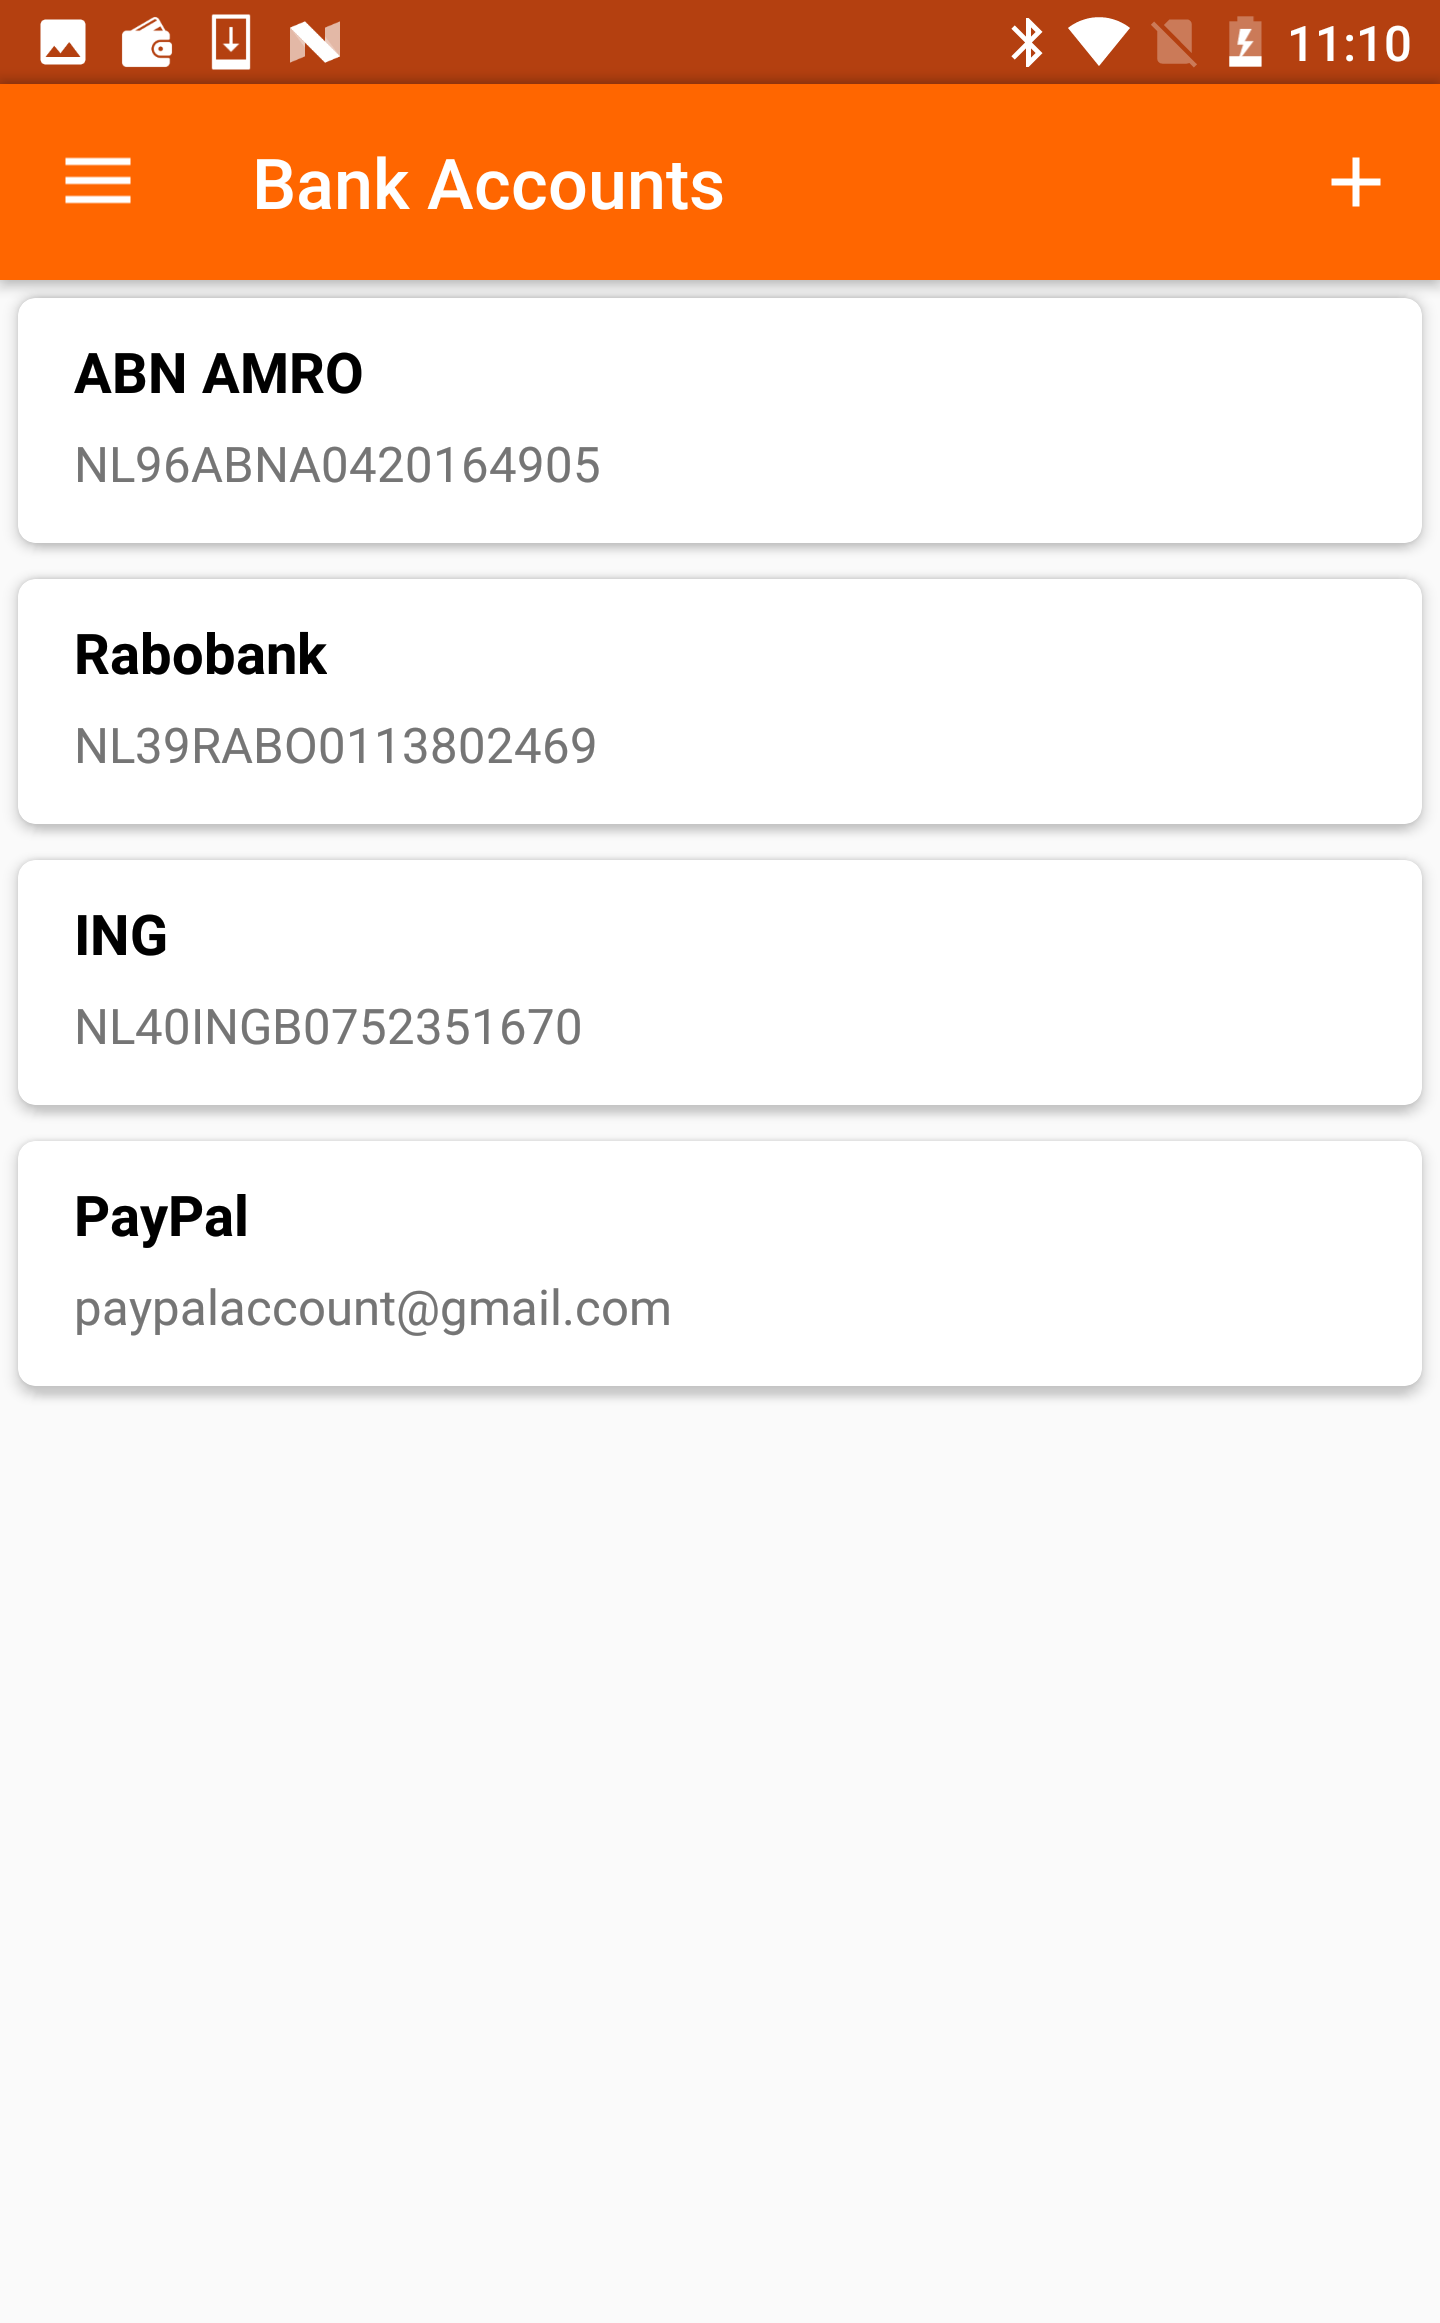
\includegraphics[width=0.48\columnwidth]{assets/android_2.png}
%	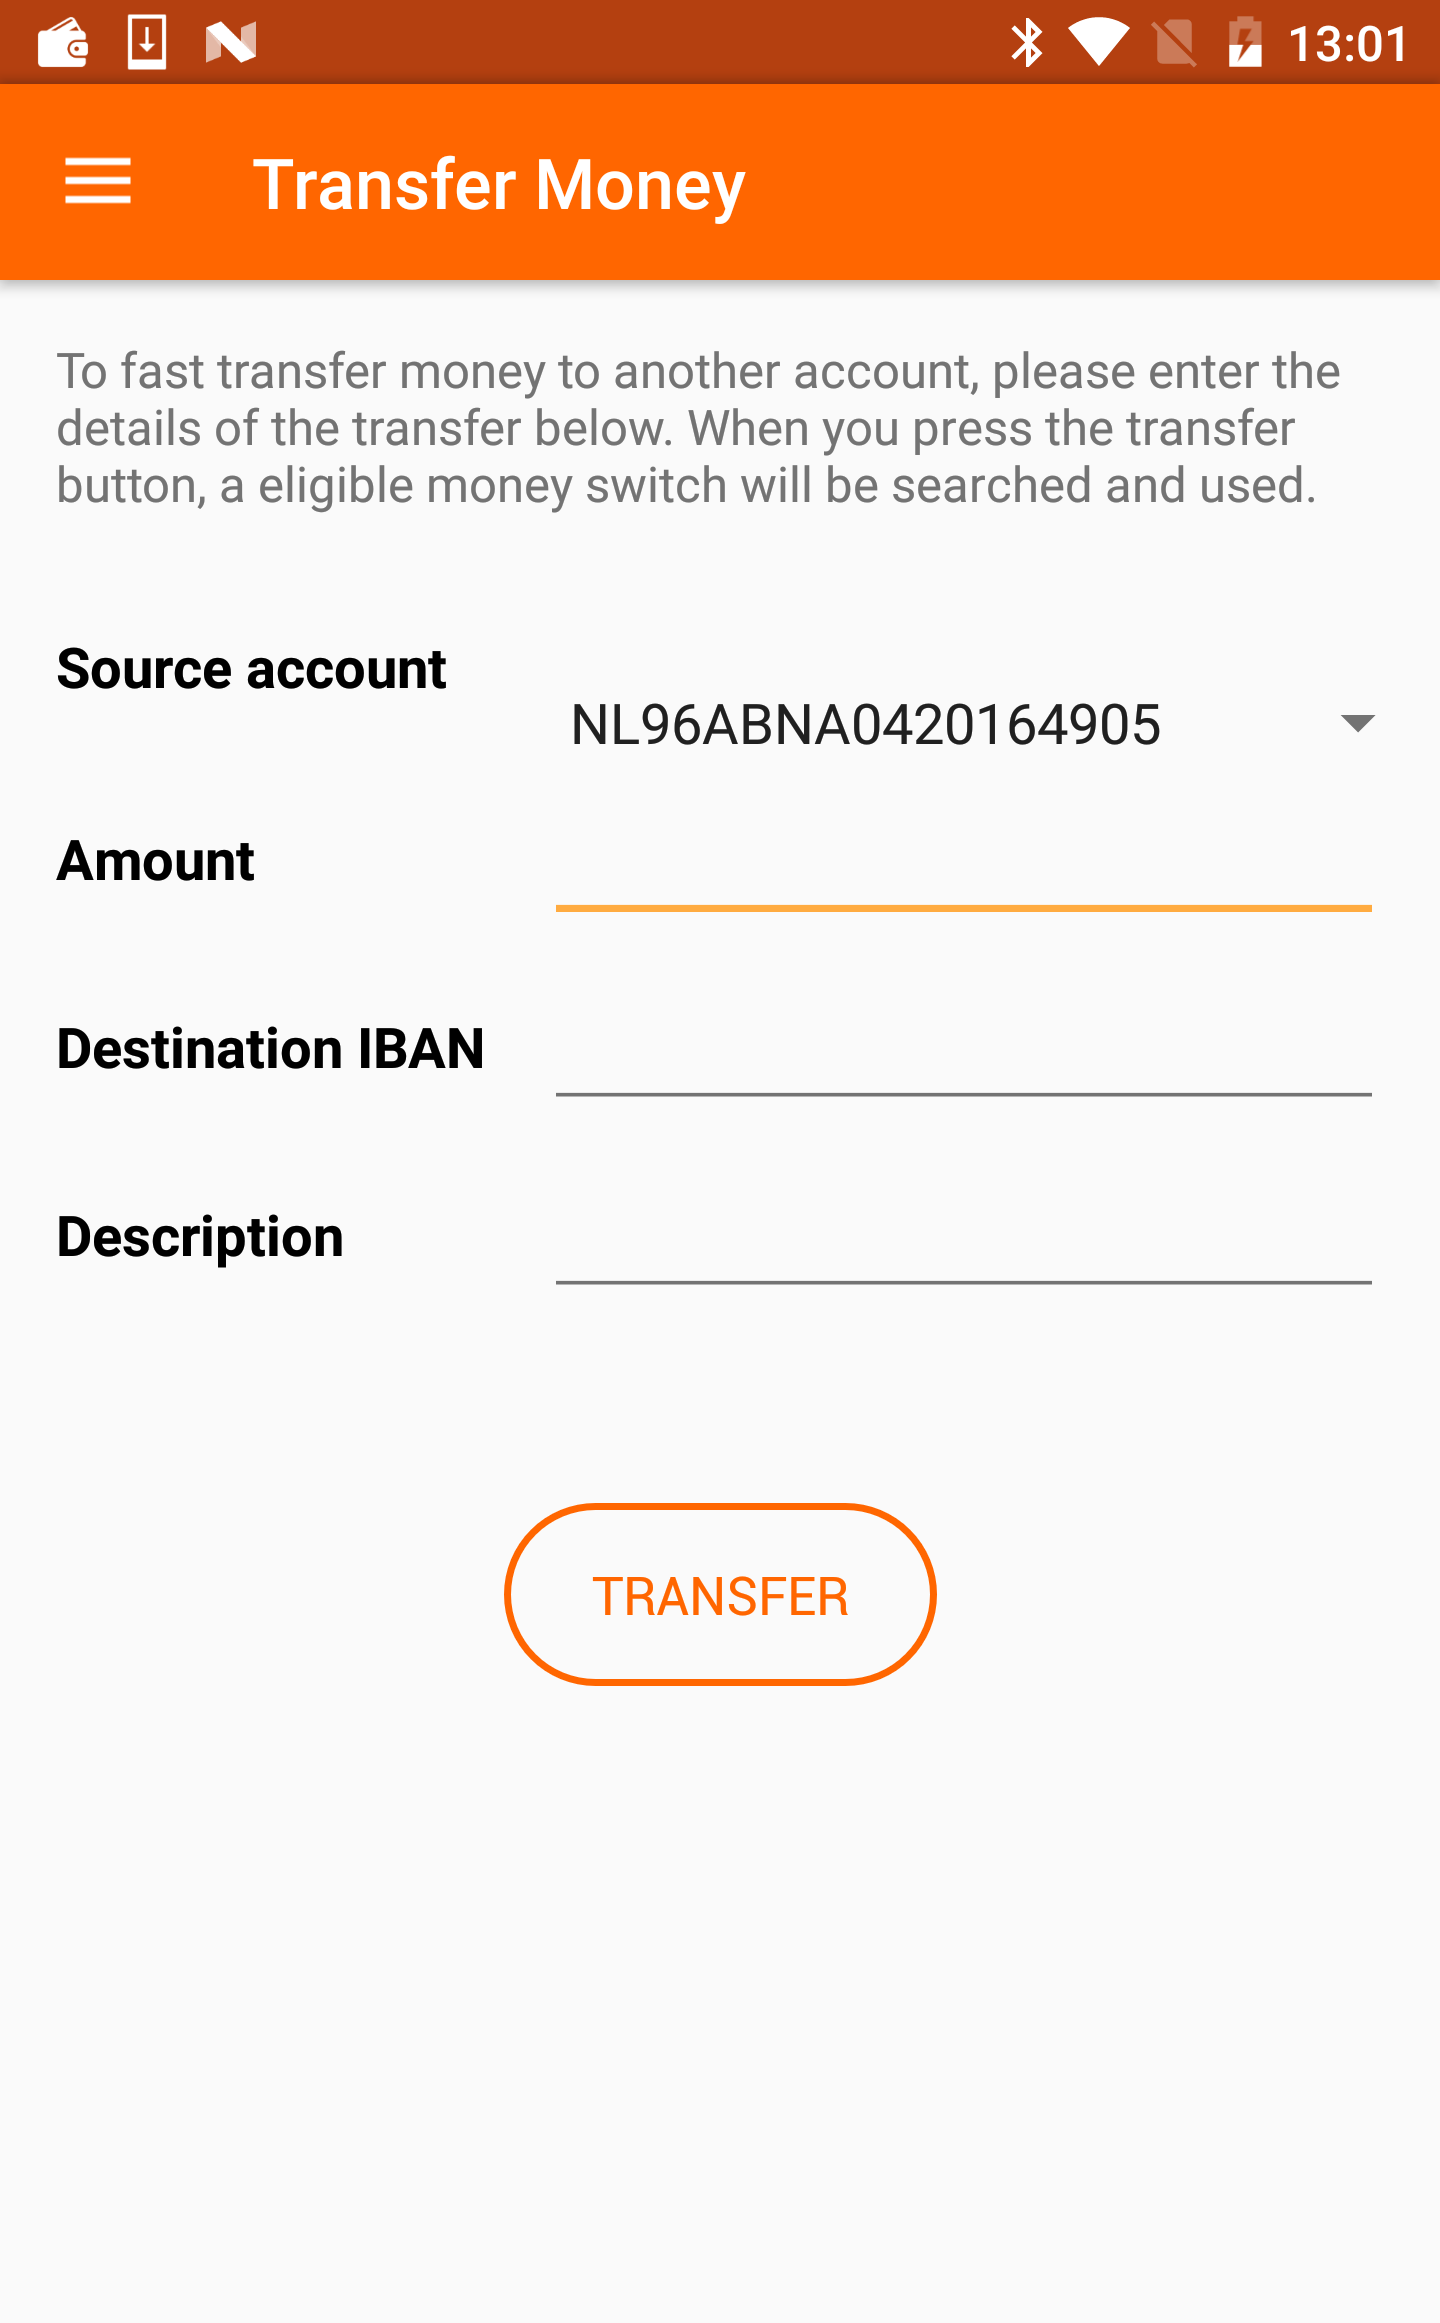
\includegraphics[width=0.48\columnwidth]{assets/android_1.png}
%	\caption{The Internet-of-Money application for Android.}
%	\label{fig:android_app}
%\end{figure}

\subsubsection*{Scalability}
Our overlay network is scalable, due to the absence of global consensus.
However, techniques like incremental settlement lead to additional payments and a higher load on the banks.
In addition, the choice of reputation mechanism used in Internet-of-Money influences scalability.

\section{Related Work}
% blockchain-based solutions
The last few years, there has been a steep increase in Fintech start-ups, eager to disrupt existing financial services.
Hawala is an informal system to transfer value, without actually moving money~\cite{jost2003hawala}.
It consists of a network of hawala brokers, that take a small commission.
In contrast to our system, trust in hawala is cultivated in an analogue manner whereas our model depends on a digital solution.

Innovation in the financial sector has been catalysed by the popularity of Blockchain technology, aiming to build trust between strangers without involvement of centralized authorities.
Bitcoin has proven that a sustainable currency can be built without a central bank in control~\cite{nakamoto2008bitcoin}.
However, wide-spread adoption stays out due to its volatile pricing, high transaction fees, relatively slow confirmation times and unsure future.
The Lightning Network aims to improve scalability of Bitcoin by providing bi-directional payment channels between users~\cite{poon2015bitcoin}.
Payments between two users not directly connected with a payment channel, are realised by routing payments through channels of other users.
This has similarities with money routing in Internet-of-Money.
New usages of blockchain technology are focussed around the way users transfer money and other assets.
%Byteball is a decentralized system that creates a directed, acyclic graph that stores units of value and uses an internal currency that should be paid when adding data to the global database~\cite{churyumov2016byteball}.
The Ripple project, supported by various major banks, attempts to build a connected network of financial institutions and payment providers~\cite{schwartz2014ripple}.
Their solution aims to significantly speed up traditional money transfers, lower costs and provide support for high-volume transactions.
R3 Corda can be compared to TrustChain since they share the idea that a ledger with global consistency is often not necessary~\cite{brown2016introducing}.

While blockchain solutions are slowly being adopted, the aforementioned systems all aim to increase utility by building a financial network from scratch.
In comparison, Internet-of-Money is built upon existing, proven infrastructure, making migration towards our system effortless.
%In particular, users are able to operate in the network by using payment primitives familiar to them.
%In particular, users act in the network with currencies supported by their banks and do not have to convert between unfamiliar assets.

%Tor, an overlay network to provide anonymous communication between entities in a network, uses a mechanism similar to money circuits and intermediate nodes.
%This mechanism, also called \emph{onion routing}, routes encrypted data over a circuit of nodes to guarantee privacy.

%The generic problem of establishing trust between strangers has been researched for decades.
%The work of Castelfranchi et al. use a cognitive approach to shed light on the notion of social trust and define trust both as a mental state and as a social attitude and relation. % https://www.researchgate.net/publication/267260663_Social_Trust_A_Cognitive_Approach
%Paul Marsh formalises trust as a computational concept and presents a formalism for trust which provides the reader with a tool for precise discussion, ready to be embedded in an artificial agent.
%Many researchers tried to establish trust using reputation mechanisms, however, a generic solution stays out~\cite{delaviz2012sybilres}\cite{kamvar2003eigentrust}\cite{srivatsa2005trustguard}\cite{post2011bazaar}.

% Sybil resistance of reputation mechanisms

\begin{figure}[t]
	\centering
	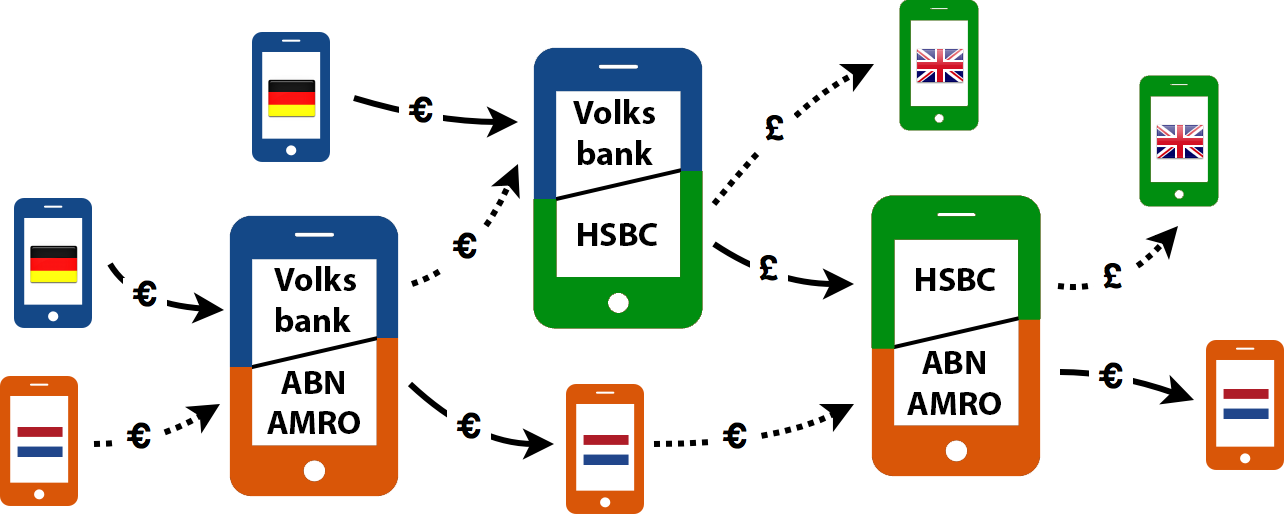
\includegraphics[width=1\textwidth]{iom/assets/internet_of_money_network.png}
	\caption{Fast international money transfers and currency conversion using Internet-of-Money. Distinct money circuits are indicated by different arrow styles.}
	\label{fig:internet_of_money_network}
\end{figure}

\section{Conclusions}
We explored a new stage in the evolution of digital trust and addressed the problem of trusting strangers with your money.
The tamper-proof TrustChain structure provides a scalable and public trace of historical interactions, and allows detection and punishment of potential fraud.
We expand upon this with an overlay network to transfer money within seconds to others, using other network participants as financial intermediaries.
This mechanism depends on the fast settlement of in-house payments.
%No changes to existing infrastructure is required to support this idea.
Our open ecosystem dramatically improves speed when initiating cross-border payments while preserving privacy and scalability.
Our experiments demonstrated the efficiency of in-house payments and effectiveness of money routers.
Additionally, we have proven that our fraud detection mechanism, together with incremental settlement and multi-flow payments, limits misuse and punishes malicious behaviour.
However, there are various legal issues and limitations that should be addressed, mostly by financial institutions, before broader usage can be realised.

This work is an important milestone in our ambitious vision to create the \emph{programmable economy}.
Ongoing work towards this goal addresses self-sovereign identity, scalable blockchain consensus compatible with TrustChain, and decentralized marketplaces.
Upcoming experimentation will focus on expanding Internet-of-Money to support additional banks, currency conversion and international bank transfers.
For this experiment, we utilize additional type of money switches to send money across the globe in seconds.
This structure is presented in Figure \ref{fig:internet_of_money_network} and is the first step towards fast and trusted international payments.